\newcommand{\precDTL}{5} % TODO choose something larger than k for smallest 1e-k
                         %      ever seen in plots
In diesem abschließenden Kapitel möchten wir nun die in
\Cref{chap:implementation} beschriebene Realisierung von
\Cref{alg:primalDualIteration} mit Abbruchkriterium
\eqref{eq:terminationCriterion} im Solve-Schritt der AFEM-Schleife aus
\Cref{fig:afemLoop} an einigen Benchmark-Problemen untersuchen.
Dabei benutzen wir die Bezeichnungen aus \Cref{alg:primalDualIteration} und
schreiben $\ucrt$ für $\ucr$ sowie $\bar\Lambda_{0,\Tcal}$ für $\bar\Lambda_0$
aus \Cref{thm:convergenceIteration} bezüglich einer Triangulierung $\Tcal$ .
Zunächst möchten wir alle Parameterwahlen aufführen, die in allen 
Experimenten gleich gesetzt werden, sofern nicht anders angegeben.
Als Startwert für die Iteration auf dem ersten Level wählen wir
$u_0\equiv 0$ und auf den darauffolgenden Leveln eine Prolongation wie zum
Ende von \Cref{sec:programFlow} beschrieben, womit die Wahl des Startwerts
der ersten Levels keinen nennenswerten Einfluss auf die Dauer des Experiments
oder die Güte der Ergebnisse hat. 
Für jeden Aufruf der primalen-dualen Iteration wählen wir $\Lambda_0$ wie in
\Cref{eq:choiceInitialDualVariableImplementation} angegeben.
Dabei konstruieren wir Probleme, bei denen die exakte Lösung bekannt ist,
nach \Cref{sec:constructionInputSignal}. 
Bei diesen ist ein Argument $r$ stets aus $[0,\infty)$.
Als besonderes Augenemerk betrachten wir dabei zunächst zwei Eingangssignale,
um in einigen Experimenten in \Cref{sec:choiceOfParameters} die Parameter für
die primale-duale Iteration zu ermitteln, die in allen weiteren Experimenten
genutzt werden sollen.
Andere Funktionen werden wir bei Bedarf betrachten, um bestimmte Eigenschaften
zu untersuchen im Vergleich zu diesen beiden Benchmark-Problemen.
Für ein Experiment mit exakter Lösung betrachten wir für einen Parameter
$\beta\geq 1/2$, wobei wir $\beta =1$ wählen, die Funktion
\begin{align*}
  u(r)&\coloneqq
  \begin{cases}
    1, 
    & \text{falls } r\in \left[0,\frac{1}{6}\right]\!,\\
    1+(6r-1)^\beta, 
    & \text{falls } r\in \left(\frac{1}{6}, \frac{1}{3}\right]\!,\\
    2, 
    & \text{falls } r\in \left(\frac{1}{3}, \frac{1}{2}\right]\!,\\
    2\left(\frac{5}{2}-3r\right)^\beta, 
    & \text{falls } r\in \left(\frac{1}{2}, \frac{5}{6}\right]\!,\\
    0, 
    & \text{falls } r\in \left(\frac{5}{6}, \infty\right)\!,\\
  \end{cases}
\end{align*}
und wählen
\begin{align*}
  \sgn\big(\partial_r u(r)\big) 
  &\coloneqq
  \begin{cases}
    12r-36r^2, 
    & \text{falls } r\in \left[0,\frac{1}{6}\right]\!,\\
    1, 
    & \text{falls } r\in \left(\frac{1}{6}, \frac{1}{3}\right]\!,\\
    \cos(\pi(6r-2)), 
    & \text{falls } r\in \left(\frac{1}{3}, \frac{1}{2}\right]\!,\\
    -1, 
    & \text{falls } r\in \left(\frac{1}{2}, \frac{5}{6}\right]\!,\\
    -\frac{1+\cos(\pi(6r-5))}{2}, 
    & \text{falls } r\in \left(\frac{5}{6}, \infty\right)\!.
  \end{cases}
\end{align*}
Nach \Cref{eq:constructionInputSignal} ist $u$ mit dieser Wahl von
$\sgn\big(\partial_r u\big)$ die Lösung von \Cref{prob:continuousProblem} mit
Eingangssignal
\begin{align}
  \label{eq:inputSignalF01}
  f_\alpha(r)
  &=
  \begin{cases}
    \alpha-12(2-9r), 
    & \text{falls } r\in \left[0,\frac{1}{6}\right]\!,\\
    \alpha\left(1+(6r-1)^\beta\right)-\frac{1}{r}, 
    & \text{falls } r\in \left(\frac{1}{6}, \frac{1}{3}\right]\!,\\
    2\alpha+6\pi\sin(\pi(6r-2))-\frac{1}{r}\cos(\pi(6r-2)), 
    & \text{falls } r\in \left(\frac{1}{3}, \frac{1}{2}\right]\!,\\
    2\alpha\left(\frac{5}{2}-3r\right)^\beta+\frac{1}{r},
    & \text{falls } r\in \left(\frac{1}{2}, \frac{5}{6}\right]\!,\\
    -3\pi\sin(\pi(6r-5))+\frac{1+\cos(\pi(6r-5))}{2r}, 
    & \text{falls } r\in \left(\frac{5}{6}, \infty\right)\!.
  \end{cases}
\end{align}
Das Eingangssignal $f_\alpha$ für zwei Wahlen von $\alpha$ und die exakte
Lösung $u$ können in \Cref{fig:f01Plots} betrachtet werden.
Wir können anhand von \Cref{fig:f01Plots} auch feststellen, dass für große
$\alpha$ die Interpretation des ROF-Modells aus \Cref{chap:introduction}
zutrifft, denn rein optisch gilt für $\alpha=10^4$ annähernd $f_\alpha=\alpha
u$.
Ebenfalls nach \Cref{sec:constructionInputSignal} können die schwachen
Gradienten von $u$ und $f_\alpha$ bestimmt werden mithilfe der partiellen 
Ableitungen
\begin{align*}
  \partial_r f_\alpha(r)
  &=
  \begin{cases}
    108,
    & \text{falls } r\in\left[0,\frac{1}{6}\right]\!,\\
    6\alpha\beta(6r-1)^{\beta-1} +\frac{1}{r^2}, 
    & \text{falls } r\in\left(\frac{1}{6},\frac{1}{3}\right]\!,\\
    \left(36\pi^2+\frac{1}{r^2}\right)\cos(\pi(6r-2))
    + \frac{6\pi}{r}\sin(\pi(6r-2)), 
    & \text{falls } r\in\left(\frac{1}{3},\frac{1}{2}\right]\!,\\
    -\left(6\alpha\beta\left( \frac{5}{2}-3r \right)^{\beta-1}+
    \frac{1}{r^2}\right),
    & \text{falls } r\in\left(\frac{1}{2},\frac{5}{6}\right]\!,\\
    -\left( \left( 18\pi^2+\frac{1}{2r^2} \right)\cos(\pi(6r-5))
    +\frac{1}{2r^2} + \frac{3\pi}{r}\sin(\pi(6r-5))\right)\!, 
    &\text{falls } r\in\left(\frac{5}{6},\infty\right)\!,
  \end{cases}
\end{align*}
und 
\begin{align*}
  \partial_r u(r) 
  &= 
  \begin{cases}
    0,
    & \text{falls } r\in\left[0,\frac{1}{6}\right]\!,\\
    6\beta(6r-1)^{\beta-1}, 
    & \text{falls } r\in\left(\frac{1}{6},\frac{1}{3}\right]\!,\\
    0, 
    & \text{falls } r\in\left(\frac{1}{3},\frac{1}{2}\right]\!,\\
    -6\beta\left( \frac{5}{2}-3r \right)^{\beta-1},
    & \text{falls } r\in\left(\frac{1}{2},\frac{5}{6}\right]\!,\\
    0,
    &\text{falls } r\in\left(\frac{5}{6},\infty\right)\!.
  \end{cases}
\end{align*} 
Durch Kenntnis des schwachen Gradienten von $u$ erhalten wir
für die exakte Energie die Approximation
$
\DTLloaddb{db}{data/paramsReducedStandardF01.csv}
\DTLassign{db}{1}{\exactEnergy=exactEnergy} 
\DTLgdeletedb{db}
E(u)\approx\DTLround{\exactEnergy}{\exactEnergy}{\precDTL}\exactEnergy
$ für das Experiment mit $\alpha=1$ und
$
\DTLloaddb{db}{data/paramsReducedStandardF01Alpha1e4.csv}
\DTLassign{db}{1}{\exactEnergy=exactEnergy} 
\DTLgdeletedb{db}
E(u)\approx\DTLround{\exactEnergy}{\exactEnergy}{\precDTL}\exactEnergy
$ für das Experiment mit $\alpha=10^4$,
mit denen wir die jeweiligen Ergebnisse der Experimente vergleichen können.
\begin{figure}[p]
  \centering
  \begin{subfigure}[b]{.48\linewidth}
    \centering
    \caption{$f_1$}
    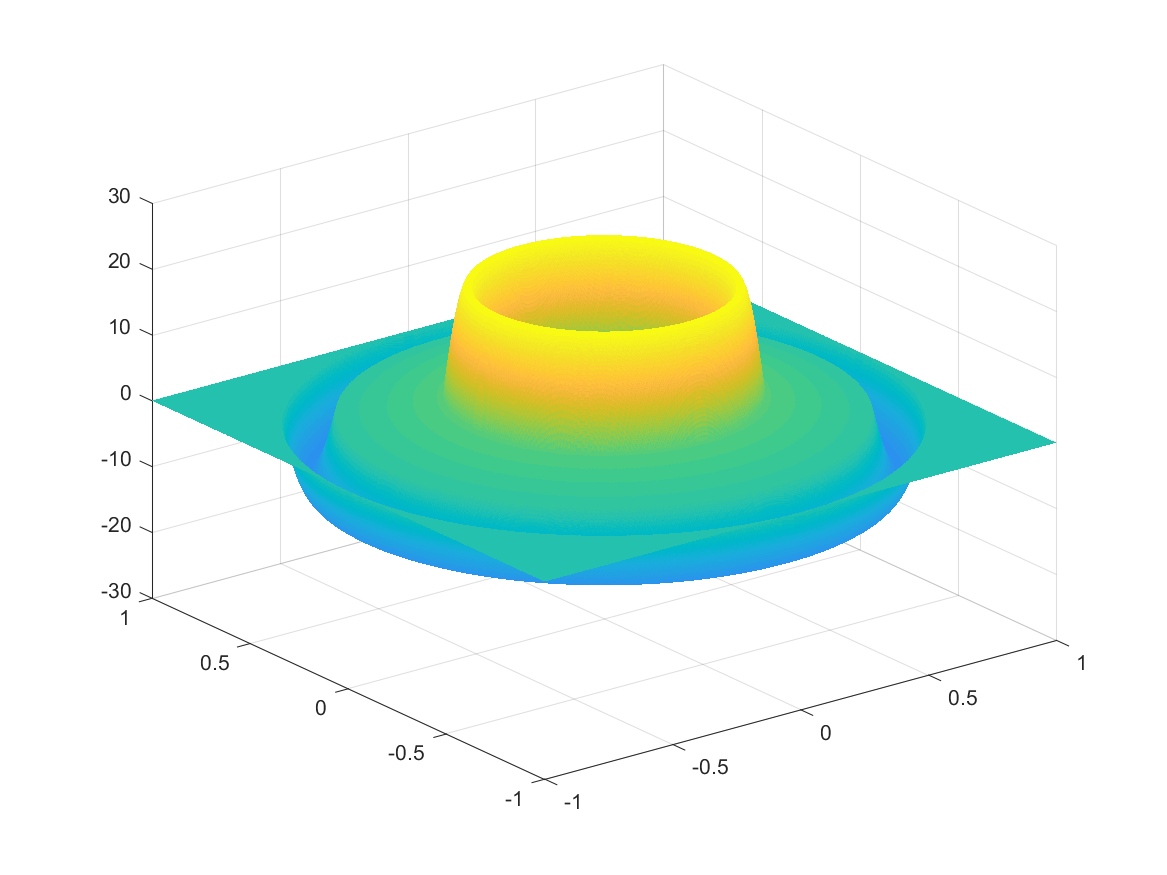
\includegraphics[trim = 40 30 30 30, clip, width=\linewidth]
      {pictures/chapExperiments/secGeneralInfo/f01Plots/inSi1.png}
    \label{fig:f01InSi}
  \end{subfigure}
  \quad
  \begin{subfigure}[b]{.48\linewidth}
    \centering
    \caption{$f_1$ entlang der x- und y-Achse}
    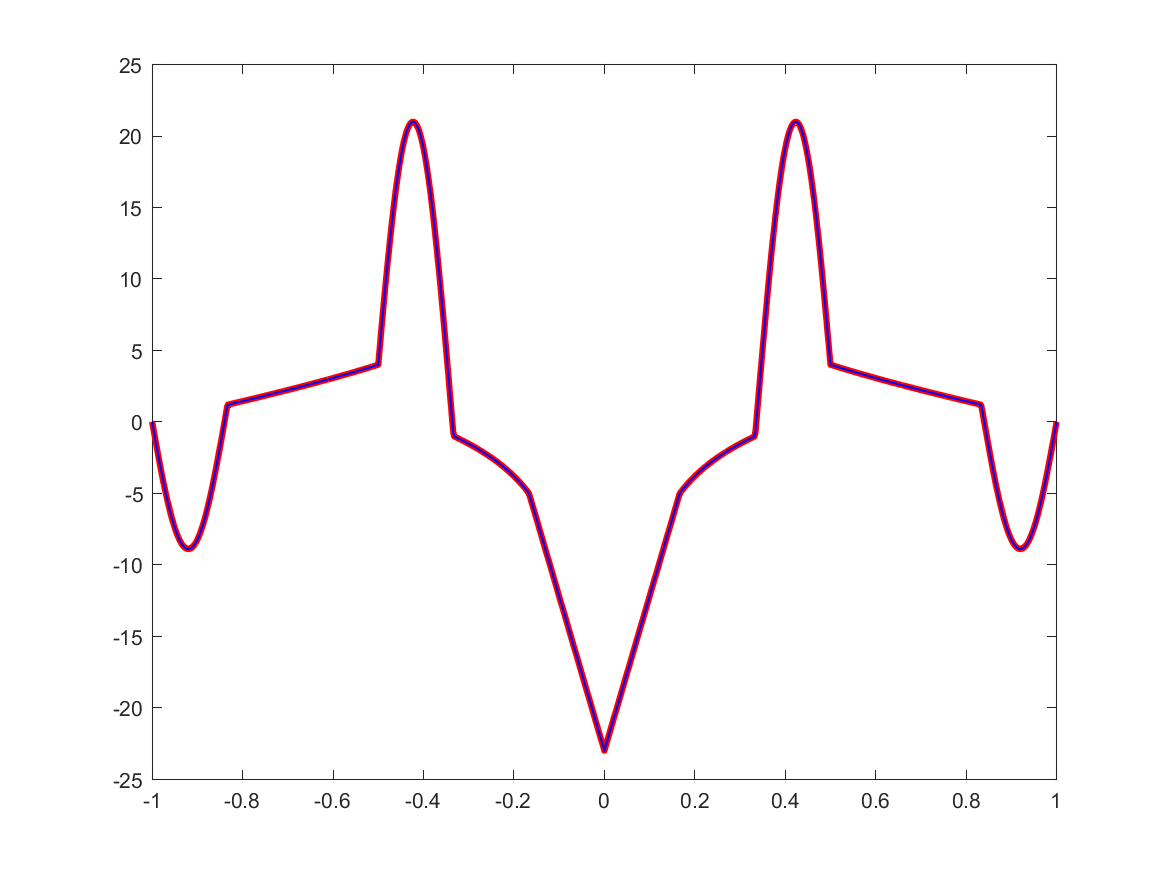
\includegraphics[trim = 50 30 50 20, clip, width=\linewidth]
      {pictures/chapExperiments/secGeneralInfo/f01Plots/inSi1Axis.png}
    \label{fig:f01InSiAxis}
  \end{subfigure}

  \begin{subfigure}[b]{.48\linewidth}
    \centering
    \caption{$f_{10^4}$}
    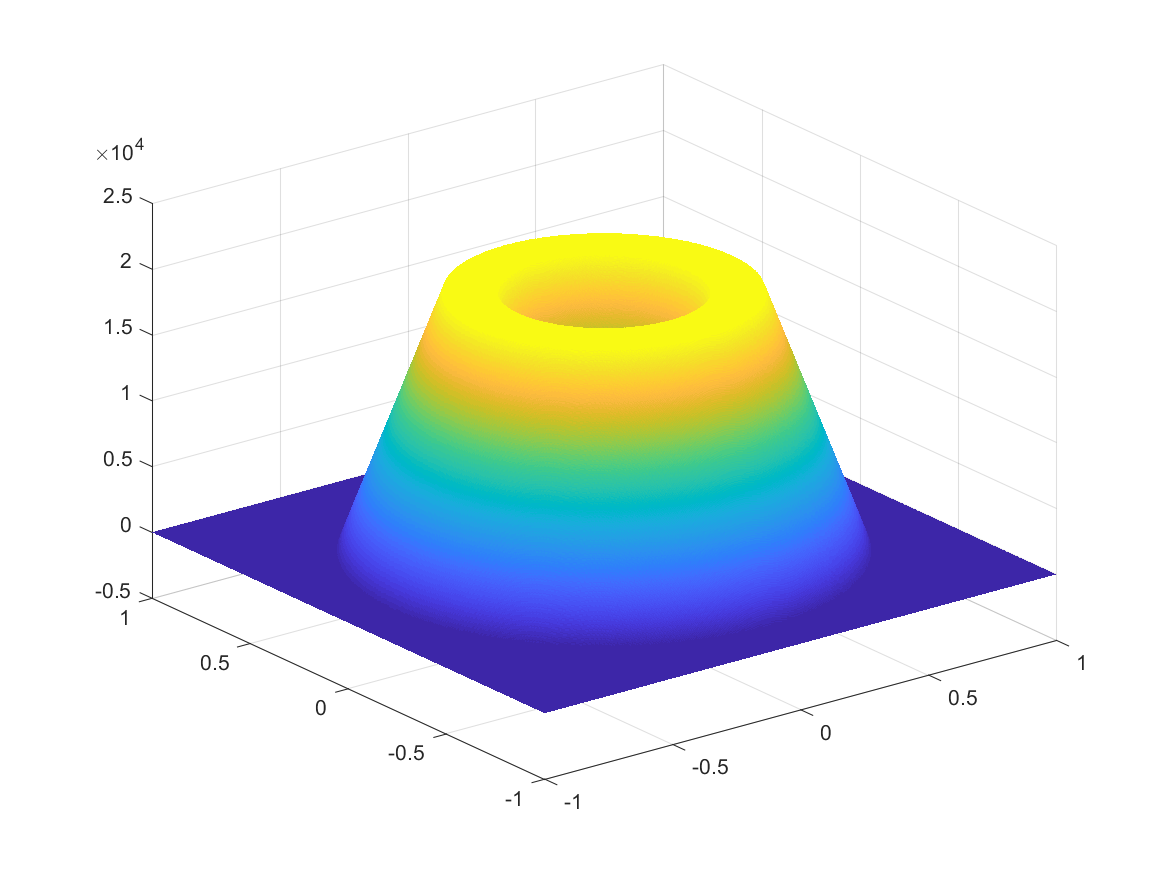
\includegraphics[trim = 40 30 30 30, clip, width=\linewidth]
      {pictures/chapExperiments/secGeneralInfo/f01Plots/inSi1e4.png}
    \label{fig:f01AlphaLargeInSi}
  \end{subfigure}
  \quad
  \begin{subfigure}[b]{.48\linewidth}
    \centering
    \caption{$f_{10^4}$ entlang der x- und y-Achse}
    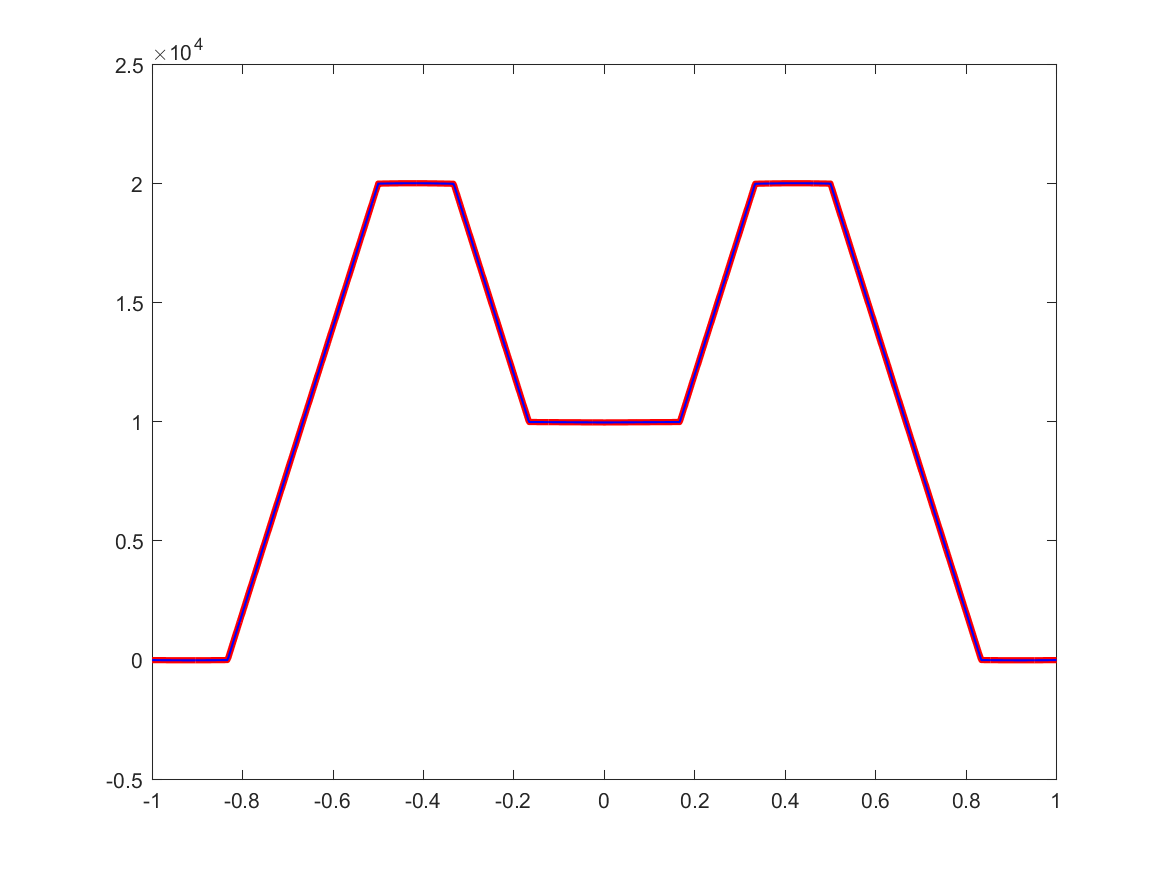
\includegraphics[trim = 50 30 50 20, clip, width=\linewidth]
      {pictures/chapExperiments/secGeneralInfo/f01Plots/inSi1e4Axis.png}
    \label{fig:f01AlphaLargeInSiAxis}
  \end{subfigure}

  \begin{subfigure}[b]{.48\linewidth}
    \centering
    \caption{$u$}
    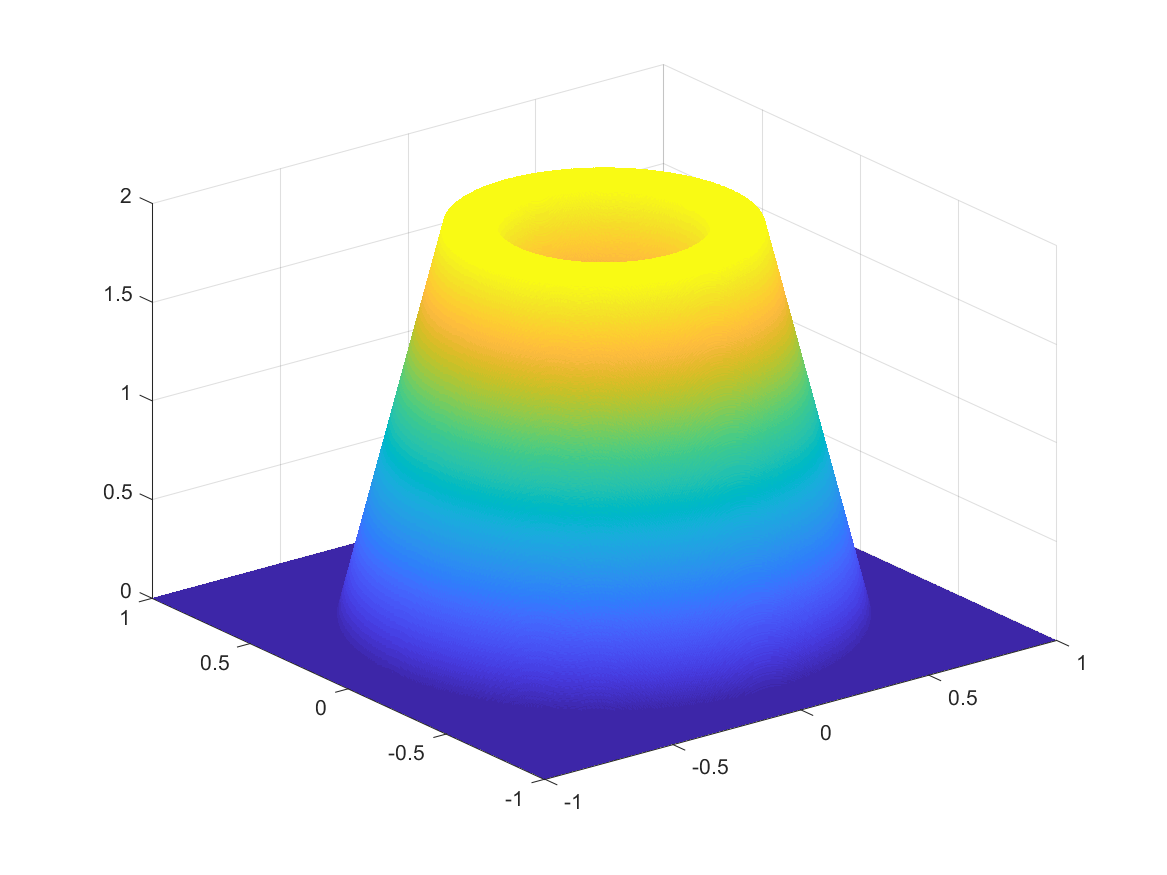
\includegraphics[trim = 40 30 30 30, clip, width=\linewidth]
      {pictures/chapExperiments/secGeneralInfo/f01Plots/exactSolution.png}
    \label{fig:f01ExactSol}
  \end{subfigure}
  \quad
  \begin{subfigure}[b]{.48\linewidth}
    \centering
    \caption{$u$ entlang der x- und y-Achse}
    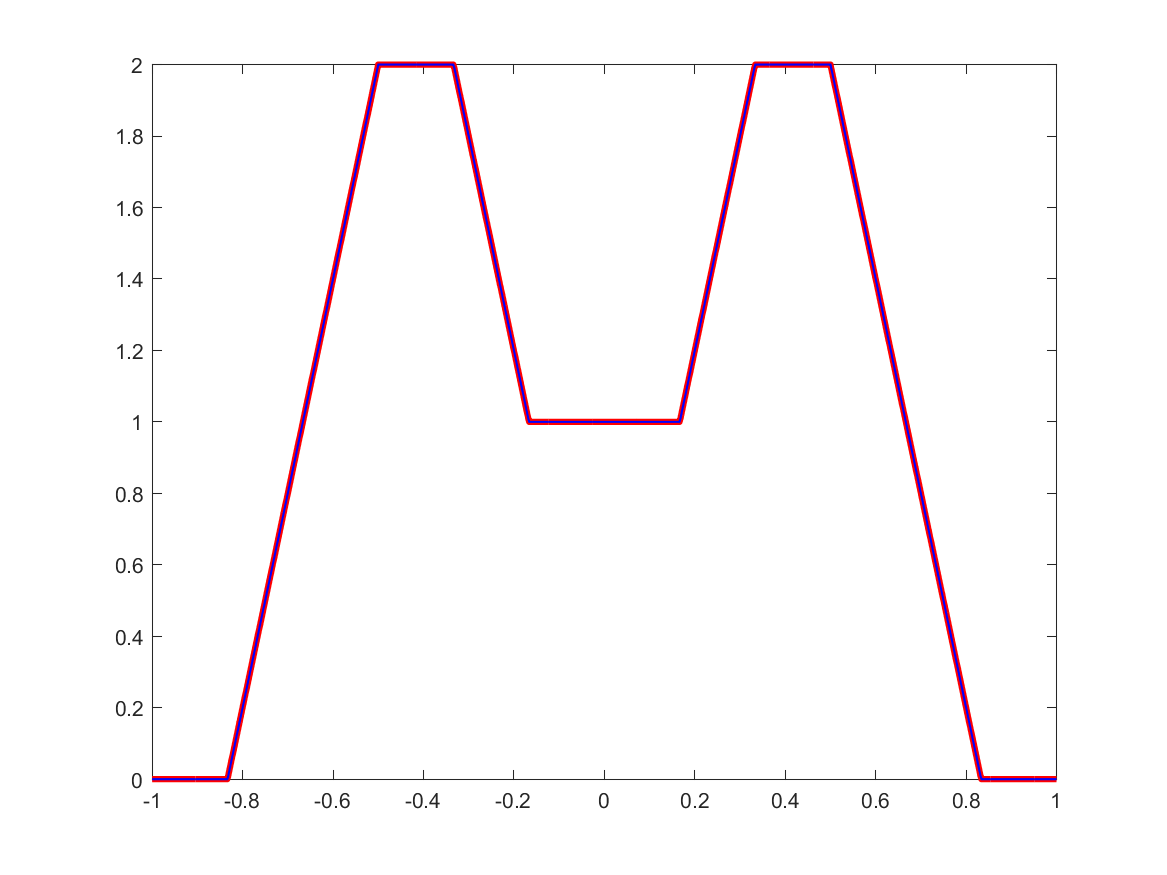
\includegraphics[trim = 50 30 50 20, clip, width=\linewidth]
      {pictures/chapExperiments/secGeneralInfo/f01Plots/exactSolutionAxis.png}
    \label{fig:f01ExactSolAxis}
  \end{subfigure} 
  \caption{Eingangssignal $f_\alpha$ und exakte Lösung $u$ sowie deren
  Darstellungen entlang der x-Achse (blau) und der y-Achse (rot) für
  $\alpha\in\{1,10^4\}$.}
  \label{fig:f01Plots}
\end{figure}
Als initiale Geometrie, das heißt die Geometrie für das erste Level des
AFEM-Al\-go\-rith\-mus, nutzen wir in den Experimenten mit exakter Lösung
\texttt{BigSquare} des AFEM-Pakets ohne initiale Rotverfeinerung, zu sehen in
\Cref{fig:triangBigSquare}, da diese den Einheitskreis, das heißt den Träger
des Eingangssignals und der exakten Lösung nach
\Cref{sec:constructionInputSignal}, enthält.
Wenn nicht anders angegeben, dann betrachten wir dieses Beispiel stets mit
$\alpha=1$, also mit Eingangssignal $f_1$. 
Diese Wahl für $\alpha$ tätigen wir auch für die anderen Probleme mit 
exakter Lösung, falls nichts anderes angegeben ist.

Für ein Problem mit unstetigem Eingangssignal legen wir besonderes
Augenmerk auf das Graufarbenbild \texttt{cameraman} aus \cref{fig:cameraman}
als Eingangssignal. 
Wir betrachten dieses Beispiel stets mit $\alpha=10^4$.
Auch für dieses komplexere Beispiel, bei der selbst eine stückweise
Beschreibung durch Polynome augenscheinlich nur schwer möglich ist, sowie in
allen weiteren Experimenten haben selbst deutlich höhere Integrationsgrade als
$10$ zu keinen veränderten Raten geführt. 
Diese Wahl des Integrationsgrads erscheint daher als ausreichend.
Da außerdem in dieser Implementierung darauf geachtet wurde, die
\texttt{integrate} Methode des AFEM-Softwarepakets \cite{Car09} nicht während
der primalen-dualen Iteration aufzurufen, hat eine möglicherweise zu hohe Wahl
des Integrationsgrads keinen relevanten Effekt auf die Programmlaufzeit und
kann somit ohne Sorge als 10 gewählt werden.
Diese Wahl des Integrationsgrads gilt nur für die Methode \texttt{errorCRL2}
des AFEM-Softwarepakets zur Berechnung des Fehlers nicht, da diese unverändert
übernommen wurde und den Grad 12 nutzt.
Fur Experiment mit Graufarbenbild als Eingangssignal nutzen wir als initiale
Triangulierung \texttt{Square} des AFEM-Softwarepakets ohne initiale
Rotverfeinerung, zu sehen in \Cref{fig:triangSquare}.

\begin{figure}[p]
  \centering
  \begin{subfigure}[b]{.48\linewidth}
    \centering
    \caption{\texttt{BigSquare}}
    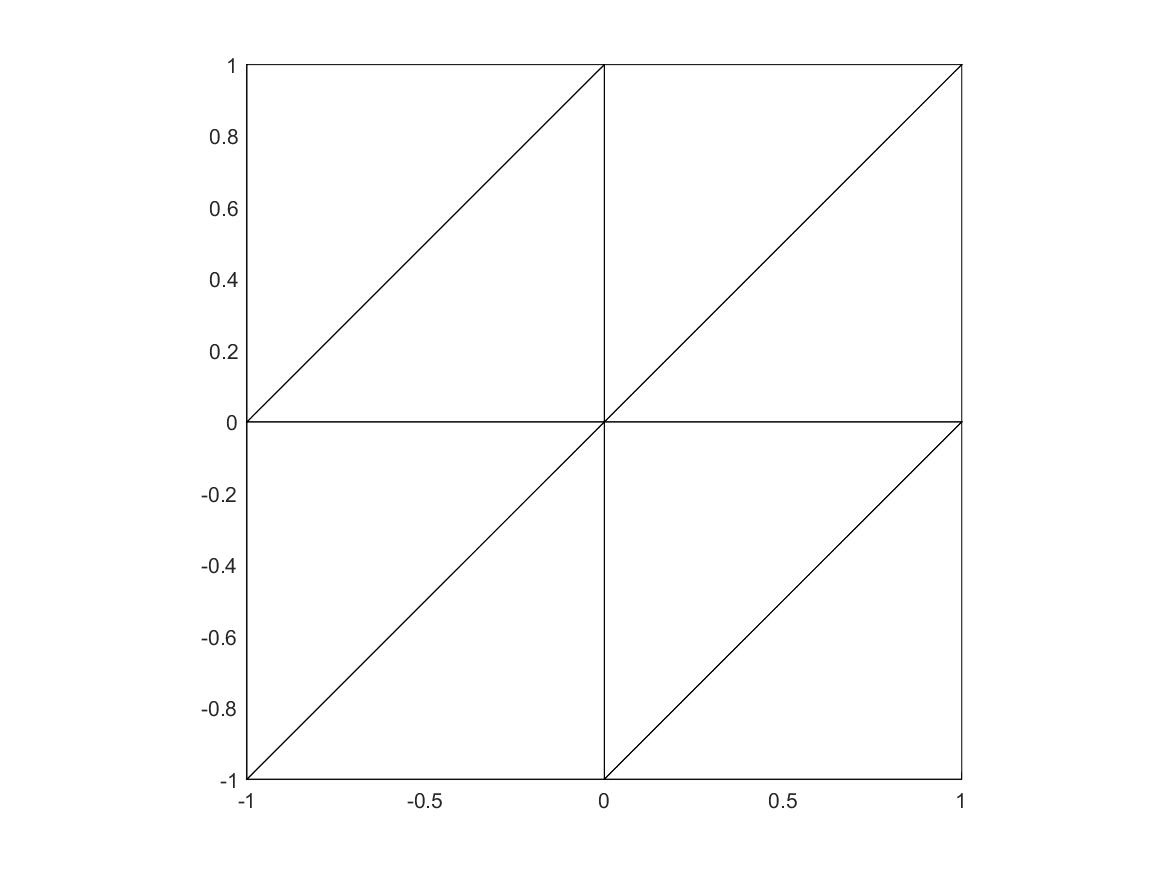
\includegraphics[trim = 90 30 90 20, clip, width=\linewidth]
      {pictures/chapExperiments/secGeneralInfo/bigSquareTriang.png}
    \label{fig:triangBigSquare}
  \end{subfigure}
  \quad
  \begin{subfigure}[b]{.48\linewidth}
    \centering
    \caption{\texttt{Square}}
    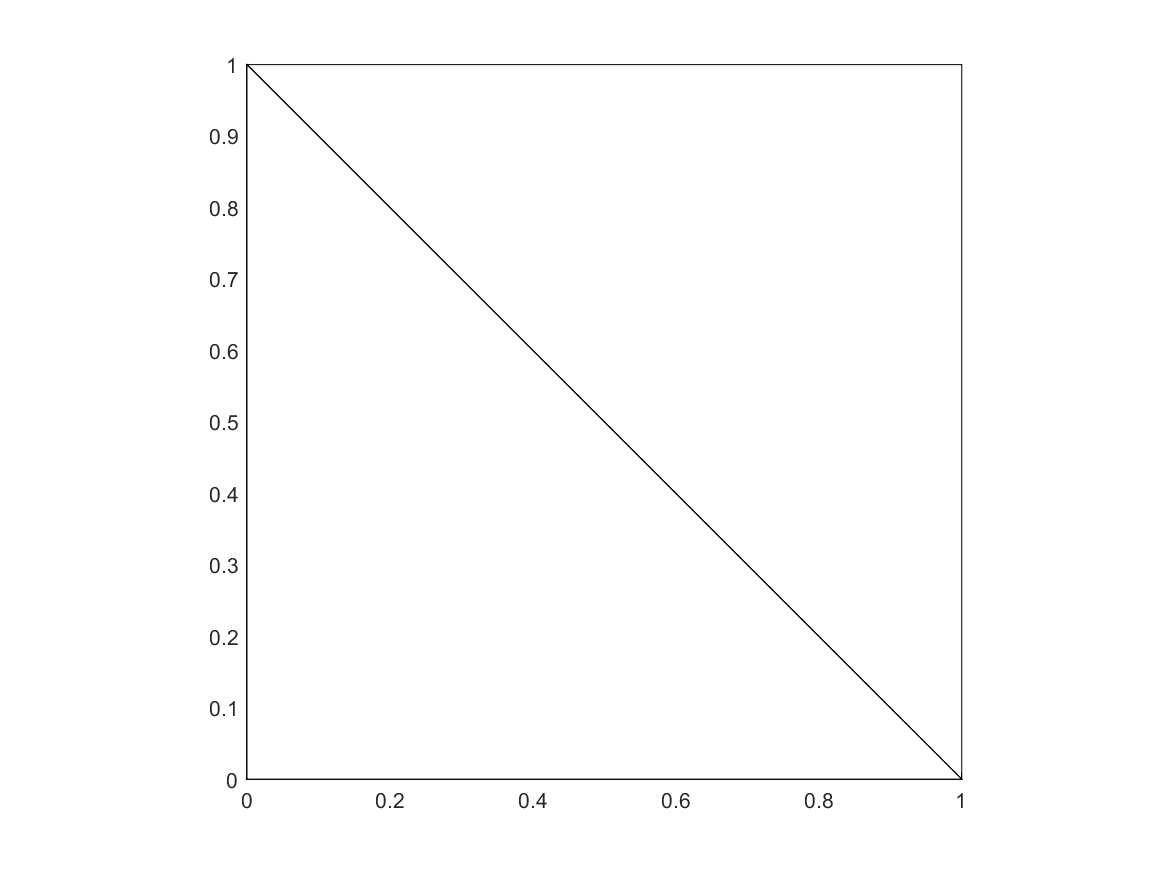
\includegraphics[trim = 90 30 90 20, clip, width=\linewidth]
      {pictures/chapExperiments/secGeneralInfo/squareTriang.png}
    \label{fig:triangSquare}
  \end{subfigure}
  \caption{In den Experimenten genutzte initiale Triangulierungen.}
  \label{fig:initialTriangulations}
\end{figure}
Führen wir ein Experiment mit adaptiver Netzverfeinerung durch, so wählen wir
den Bulk-Parameter für den Mark-Schritt des AFEM-Algorithmus $\theta=0.5$ und
den Parameter $\gamma=1$ für den Verfeinerungsindikator aus 
\Cref{def:refinementIndicator}.
Außerdem betrachten wir zur Wahl des Parameters $\gamma$ auf dem
Verfeinerungsindikator in \Cref{sec:experimentsWithExactSolution} ein
Experiment.
Auf die Wahl der Parameter $\tau$ und $\epsstop$ für die primale-duale
Iteration werden wir im folgenden \Cref{sec:choiceOfParameters} eingehen.
Die maximale Iterationszahl ist, mit Ausnahme von einem Experimente in
\Cref{sec:choiceOfParameters}, mit $10^{12}$ so gewählt, dass diese nie 
der Grund für das Beenden einer primalen-dualen Iteration ist, also stets das
Abbruchkriterium aus \eqref{eq:terminationCriterion} für den Abbruch
verantwortlich ist.
Die minimale Anzahl der Freiheitsgrade ist so gewählt, dass AFEM-Routine
manuell oder durch Server beendet wird, bevor Sie durch erreichen 
der Freiheitsgrade beendet wird. Dies geschah in allen Experimenten bei 
ungefähr $10^6$ Freiheitsgraden.

\begin{table}
  \centering
  \begin{tabular}{c|c}
    \hline
    \texttt{benchmark} & Abbildungen\\  
    \hline 
    \texttt{denoiseAlpha100} &
    \ref{fig:snr15alpha100}\\
    \texttt{denoiseAlpha1000} &
    \ref{fig:snr15alpha1000}\\
    \texttt{denoiseAlpha2500} &
    \ref{fig:snr15alpha2500}\\
    \texttt{denoiseAlpha5000} &
    \ref{fig:snr15alpha5000}\\
    \texttt{denoiseAlpha10000} &
    \ref{fig:snr15alpha10000}\\
    \texttt{denoiseAlpha50000} &
    \ref{fig:snr15alpha50000}\\
    \texttt{paramsTau\_f01\_0Dot1} &
    \ref{fig:parTauMiscF}, \ref{fig:parTauConvergence},
    \ref{fig:iterationEnergyOscillations}\\
    \texttt{paramsTau\_f01\_0Dot5} &
    \ref{fig:parTauMiscF}, \ref{fig:parTauConvergence}\\
    \texttt{standard\_f01} &
    \ref{fig:parTauMiscF}, \ref{fig:parTauConvergence}, 
    \ref{fig:iterationEnergyLevel}, \ref{fig:iterationTermination},
    \ref{fig:f01Convergence}, \ref{fig:f01SolAdaptive},
    \ref{fig:f01SupplementaryInfo}, \ref{fig:parGammaConvergence},
    \ref{fig:gamma1Triang}, \ref{fig:inSiNrIterComparison}\\
    \texttt{paramsTau\_cameraman\_0Dot1} &
    \ref{fig:parTauMiscCam}\\
    \texttt{paramsTau\_cameraman\_0Dot5} &
    \ref{fig:parTauMiscCam} \\
    \texttt{standard\_cameraman} &
    \ref{fig:parTauMiscCam}, \ref{fig:camConvergence}, \ref{fig:camTriang}\\
    \texttt{noTerminationTau\_maxIter1e5} &
    \ref{fig:parTauNoConvergence}\\
    \texttt{paramsEpsStop\_1em2} &
    \ref{fig:parEpsStopConvergence}\\
    \texttt{paramsEpsStop\_1em3} &
    \ref{fig:parEpsStopConvergence}\\
    \texttt{paramsEpsStop\_1em4} &
    \ref{fig:parEpsStopConvergence}\\
    \texttt{paramsEpsStop\_1em5} &
    \ref{fig:parEpsStopConvergence}\\
    \texttt{standardUniform\_f01} &
    \ref{fig:f01Convergence}, \ref{fig:f01SupplementaryInfo}\\
    \texttt{standard\_f01Alpha1e4} &
    \ref{fig:f01LargeAlphaConvergence}, \ref{fig:inSiNrIterComparison}\\
    \texttt{standardUniform\_f01Alpha1e4} &
    \ref{fig:f01LargeAlphaConvergence}\\
    \texttt{parGamma\_0} &
    \ref{fig:parGammaConvergence}, \ref{fig:gamma0Triang}\\
    \texttt{parGamma\_0Dot5} &
    \ref{fig:parGammaConvergence}, \ref{fig:gammaDot5Triang}\\
    \texttt{standard\_f04} &
    \ref{fig:f04Convergence}, \ref{fig:inSiNrIterComparison}\\
    \texttt{standardUniform\_f04} &
    \ref{fig:f04Convergence}\\
    \texttt{standardUniform\_cameraman} &
    \ref{fig:camConvergence}\\
    \texttt{circleContinuousAdaptive} &
    \ref{fig:circConvAdaptive}, \ref{fig:circContConvergence},
    \ref{fig:circContLvl17Triang}, \ref{fig:circContFinalTriang},
    \ref{fig:circContSol}, \ref{fig:circContSolAxis}\\
    \texttt{circleDiscontinuousAdaptive} &
    \ref{fig:circConvAdaptive}\\
    \texttt{circleContinuousUniform} &
    \ref{fig:circConvUniform}, \ref{fig:circContConvergence},
    \ref{fig:circDiscLvl17Triang}, \ref{fig:circDiscFinalTriang},
    \ref{fig:circDiscSol}, \ref{fig:circDiscSolAxis}\\
    \texttt{circleDiscontinuousUniform} &
    \ref{fig:circConvUniform}\\
    \hline
  \end{tabular}
  \caption{Eingabe \texttt{benchmark} für \texttt{startAlgorithmCR} und die
  Abbildungen, die auf den Ergebnissen des jeweiligen Experiments basieren. 
  (Abschnittsweise diese Tabelle oder eine für alle Experimente? Reihenfolge
  der Benchmarks in Nutzungsreihenfolge oder alphabetisch?)}
  \label{tab:usedBenchmarks}
\end{table} 


\section{Wahl der Parameter für die primale-duale Iteration}
\label{sec:choiceOfParameters}

Die Experimente in diesem Abschnitt zur Ermittelung der Einstellungen
für die primale-duale Iteration werden adaptiv durchgeführt und alle hier
nicht aufgeführten Parameter werden gewählt wie im vorhergehenden Abschnitt
beschrieben.
Die Eingangssignale für die Experimente sind in der Beschreibung der 
entsprechenden Abbildung angegeben.

Zunächst interessiert und die Wahl des Parameters $\tau$ in 
\Cref{alg:primalDualIteration}. 
Diesen müssen wir nach \Cref{thm:convergenceIteration} in $(0,1]$ wählen, um
Konvergenz der primalen-dualen Iteration zu garantieren.
Der Parameter $\epsstop$ wird mit $10^{-4}$ gewählt. 
Diese Wahl wird anschließend in diesem Abschnitt ebenfalls nochmal näher
betrachtet. 
\begin{figure}[p]
  \centering
  \begin{subfigure}[b]{.48\linewidth}
    \caption{Eingangssignal $f$}
    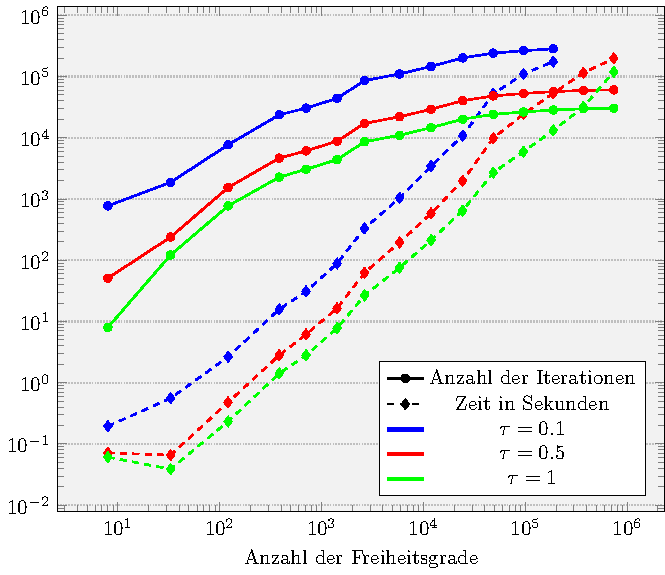
\includegraphics[width=\linewidth]
      {pictures/chapExperiments/secParameters/parTau/f01/miscF.pdf}
    \label{fig:parTauMiscF}
  \end{subfigure}
  \quad
  \begin{subfigure}[b]{.48\linewidth}
    \centering
    \caption{Eingangssignal \texttt{cameraman}}
    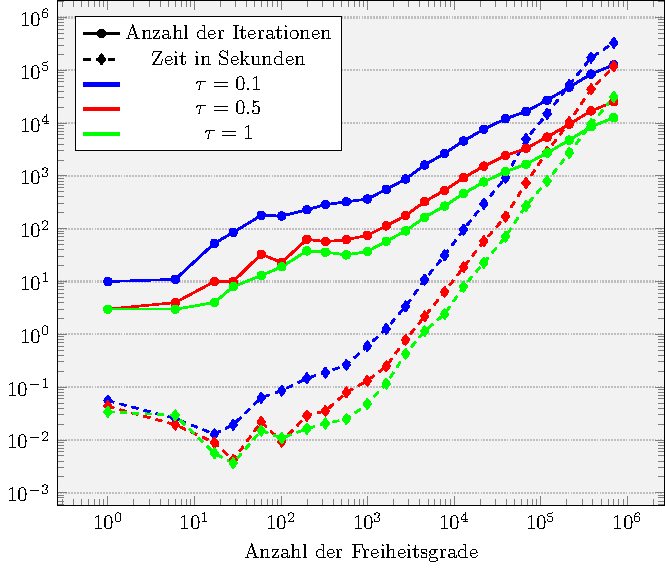
\includegraphics[width=\linewidth]
      {pictures/chapExperiments/secParameters/parTau/cam/miscCam.pdf}
    \label{fig:parTauMiscCam}
  \end{subfigure}
  \caption{Anzahl der Iterationen und benötigte Zeit für verschiedene Werte
  von $\tau$ mit den Eingangssignalen $f$ und \texttt{cameraman}.}
  \label{fig:parTauMisc}
\end{figure}
\begin{figure}[p]
  \centering
  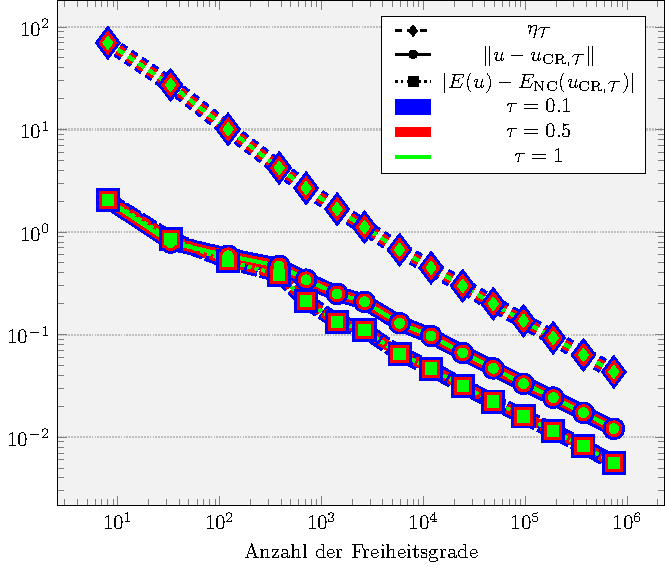
\includegraphics[width=\linewidth]
    {pictures/chapExperiments/secParameters/parTau/f01/convergenceF.pdf}
  \caption{Verfeinerungsindikator, exakter $L^2$-Fehler und Energiedifferenz 
  für verschieden Werte von $\tau$ mit Eingangangssignal $f$.}
  \label{fig:parTauConvergence}
\end{figure}
Wie in \Cref{fig:parTauMisc} zu sehen, verhält sich die Anzahl der Iteration,
und damit, wie zu erwarten war, auch die Laufzeit, antiproportional zur Größe
der hier gewählten Werte von $\tau$, d.h. größeres $\tau$ führt zu einer
geringeren Laufzeit und weniger Iterationen.
Da sich die betrachteten Graphen in \Cref{fig:parTauConvergence} für die
verschiedenen Wahlen von $\tau$ nicht sichtbar unterscheiden, schlussfolgern
wir, dass die ideale Wahl für $\tau$, die \Cref{thm:convergenceIteration}
zulässt, das heißt $\tau=1$, zu sein scheint, da die primale-duale Iteration
bei gleichen Ergebnissen für dieses $\tau$ die geringste Laufzeit hat.
Ein mögliche Erklärung liefert der Beweis von \Cref{thm:convergenceIteration}.
Die darin bewiesene \Cref{eq:upperBoundIterationError} impliziert für die
Iterate $(u_j)_{j\in\Nbb}$ auf einem Level, dass
\begin{align}
  \label{eq:nrIterationsInequality}
  \sum_{j=1}^\infty\Vert \ucrt - u_j \Vert^2 
  \leq
  \frac{1}{2\alpha\tau}
  \left(\vvvert \ucrt - u_0\vvvert^2_\nc 
  + \left\Vert \bar\Lambda_{0,\Tcal} - \Lambda_0\right\Vert^2\right)\!. 
\end{align}
Die rechte Seite ist antiproportional zu $\tau>0$, womit womöglich
die Folge $(\left\Vert \ucr - u_j\right\Vert)_{j\in\Nbb}$ schneller gegen $0$
konvergiert und damit auch das Abbruchkriterium \eqref{eq:terminationCriterion}
nach einer geringeren Anzahl von Iterationen erfüllt ist. 
Der Beweis von \Cref{thm:convergenceIteration} liefert uns keine
Informationen darüber, ob möglicherweise auch eine Wahl $\tau>1$ immer noch die
Konvergenz der primalen-dualen Iteration garantiert.
Wie aber in \Cref{fig:parTauNoConvergence} zu sehen, haben wir schon für
$\tau=1.2$ ein Beispiel gefunden, bei dem nicht davon ausgegangen werden kann,
dass die primale-duale Iteration konvergiert.
Diese Iteration wurde auf der Triangulierung aus \Cref{fig:triangBigSquare} 
durchgeführt. 
Dabei wurde die Iteration nach $10^5$ Iterationen, wie in
\Cref{fig:parTauNoConvergenceUpdates} zu sehen, abgebrochen, da kein anderes
Verhalten mehr zu erwarten war, zumal selbst für die nach
\Cref{fig:parTauMiscF} suboptimale Wahl $0.1$ für $\tau$ weniger also $10^3$
Iterationen auf der gleichen Triangulierung benötigt wurden und für die Wahl
$\tau=1$ sogar weniger als $10$ Iterationen.
\begin{figure}[p]
  \centering
  \begin{subfigure}[b]{.48\linewidth}
    \centering
    \caption{Mussugen der Updates}
    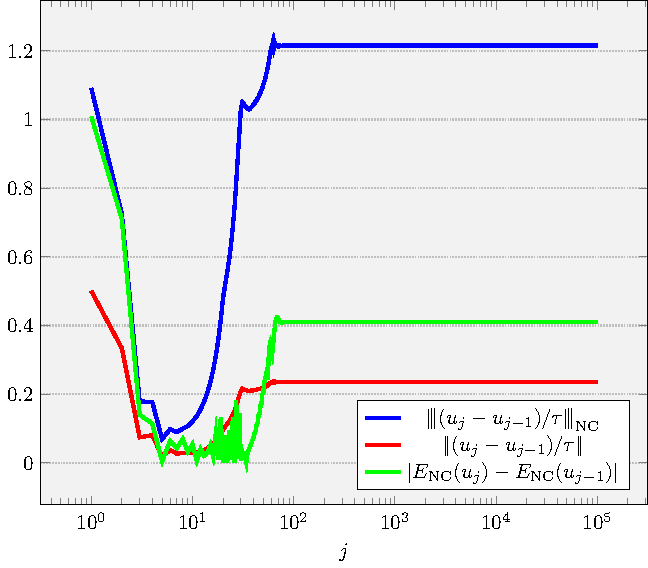
\includegraphics[width=\linewidth]
      {pictures/chapExperiments/secParameters/parTau/f01NoConv/1Dot2/convIter.pdf}
    \label{fig:parTauNoConvergenceUpdates}
  \end{subfigure}
  \quad
  \begin{subfigure}[b]{.47\linewidth}
    \centering
    \caption{Verlauf der Energie}
    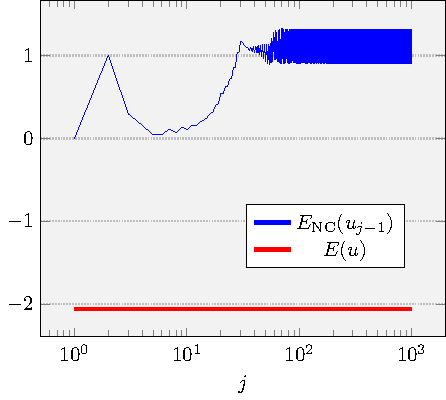
\includegraphics[width=\linewidth]
      {pictures/chapExperiments/secParameters/parTau/f01NoConv/1Dot2/convEnergy.pdf}
    \label{fig:parTauNoConvergenceEnergy}
  \end{subfigure}
  \caption{Drei Messungen des Updates der Iteration (a) und Verlauf der
  Energie während der erstens $1000$ Iterationen (b) für $\tau=1.2$ mit
  Eingangangssignal $f$.}
  \label{fig:parTauNoConvergence}
\end{figure}
Auch die Betragsdifferenz zwischen den Energien zweier Iterate stagniert.
Es ist stark davon auszugehen, dass dieses Problem mit keinem von den
Iteraten abhänigen Abbruchkriterium terminiert.
Mit \Cref{fig:parTauNoConvergenceEnergy} steht außerdem fest, dass der
Abstand zwischen den Iteraten nicht stagniert, während die Iterate divergieren
oder konvergieren, sondern dass die Iterate sich mit alternierender Energie
entwickeln zu scheinen.
Insbesondere bleibt festzuhalten, dass die von \Cref{thm:convergenceIteration}
für $\tau\in(0,1]$ garantierte Konvergenz für $\tau=1.2$ nicht eintritt.

Nun betrachen wir die Wahl des Parameteres $\epsstop$ für das Abbruchkriterium
aus \eqref{eq:terminationCriterion}.
\begin{figure}[p]
  \centering
  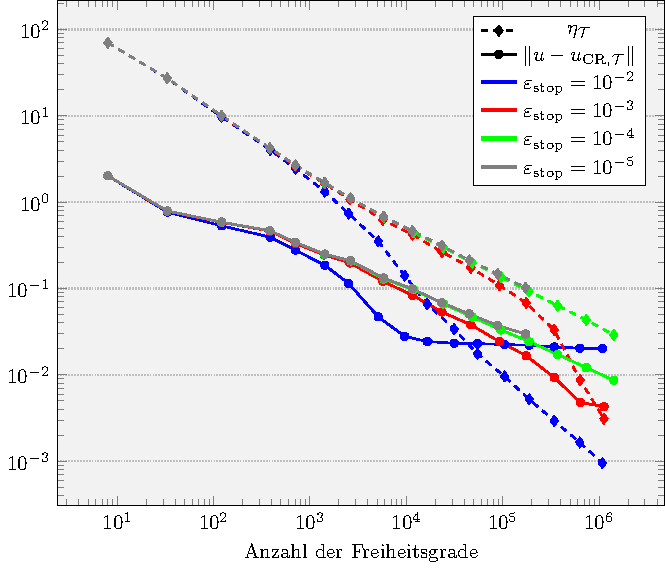
\includegraphics[width=\linewidth]
    {pictures/chapExperiments/secParameters/parEpsStop/f01/convergenceF.pdf}
  \caption{Verfeinerungsindikator und exakter $L^2$-Fehler für verschieden
  Werte von $\epsstop$ mit Eingangangssignal $f$.}
  \label{fig:parEpsStopConvergence}
\end{figure}
Wie in \Cref{fig:parEpsStopConvergence} zu sehen, stagniert der 
exakte $L^2$-Fehler für $\epsstop=10^{-2}$ und, es lässt sich erahnen, dass
dieser Effekt auch für $\epsstop=10^{-3}$ einsetzt. 
Da der Effekt bis $10^6$ Freiheitsgrade für $\epsstop\in\{10^{-4},10^{-5}\}$
noch nicht einsetzt, scheint dies an einem zu frühen Abbruch der Iteration 
durch eine zu große Toleranz $\epsstop$ zu liegen. 
Bei hohen Freiheitsgraden und einer entsprechend kleinen Netzweite muss
also $\epsstop$ ausreichend klein gewählt werden.
Da wir in den Experimenten  $10^6$ Freiheitsgrade nicht deutlich überschreiten
und sich bis dahin die Ergebnisse für die Wahlen $10^{-4}$ und $10^{-5}$ kaum
unterscheiden, die Wahl $10^{-5}$ aber eine wesentlich längere Laufzeit
verursacht, wählen wir als Standard $\epsstop=10^{-4}$.
Weiterhin bleibt festzuhalten, dass der Verfeinerungsindikator trotzdem noch
passend Dreiecke auswählt und weiter fällt, d.h. insbesondere nicht
stagnariert, auch bei stagnierendem Fehler.


\section{Experimente mit bekannter exakter Lösung}
\label{sec:experimentsWithExactSolution}

In diesem Abschnitt möchten wir nun anhand des Experiments mit Eingangssignal
$f$ aus \Cref{eq:inputSignalF01} die Ergebnisse des Programms.
Außerdem werden wir die Ergebnisse mit zwei weiteren Eingangssignalen,
für die exakte Lösungen bekannt sind, vergleichen, um so weitere Aussagen
über die Ergebnisse treffen zu können.
Die Wahl aller Parameter, die hier nicht noch einmal aufgeführt werden, ist
im einleitenden Teil und dem vorherigen \Cref{sec:choiceOfParameters} 
begründet worden.
Zunächst möchten wir anhand der Experimente mit Eingangssignal $f$ einige
Eigenschaften der primalen-dualen Iteration betrachten.

\begin{figure}[p]
  \centering
  \begin{subfigure}[b]{.5\linewidth}
    \centering
    \caption{Energieverlauf der Iterationen per Level}
    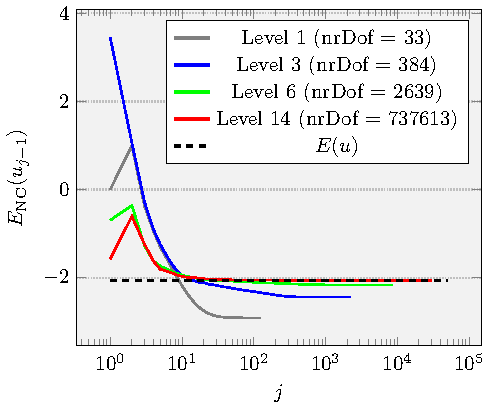
\includegraphics[width=\linewidth]
      {pictures/chapExperiments/secExactSol/iteration/lvlWise/convEnergy.pdf}
    \label{fig:iterationEnergyLevel}
  \end{subfigure}
  \quad
  \begin{subfigure}[b]{.46\linewidth}
    \centering
    \caption{Oszillierendes Beispiel}
    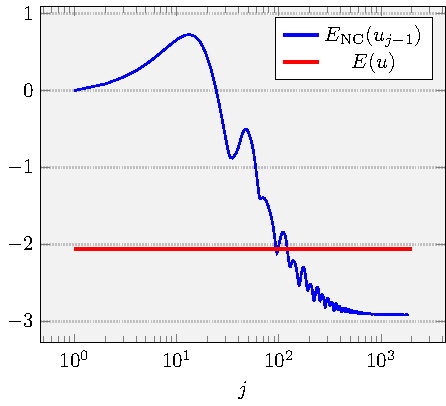
\includegraphics[width=\linewidth]
      {pictures/chapExperiments/secExactSol/iteration/osc/convEnergy.pdf}
    \label{fig:iterationEnergyOscillations}
  \end{subfigure}
  \caption{Energieentwicklung während der primalen-dualen Iteration für
  Eingangssignal $f$ auf verschiedenen Leveln mit $\tau=1$ (a) und für ein
  Level mit $\tau=10^{-1}$ (b) wobei das initale Level 0 ist.}
  \label{fig:iterationEnergy}
\end{figure}

\begin{figure}[p]
  \centering
  \begin{subfigure}[b]{.5\linewidth}
    \centering
    \caption{Updatenorm per Level}
    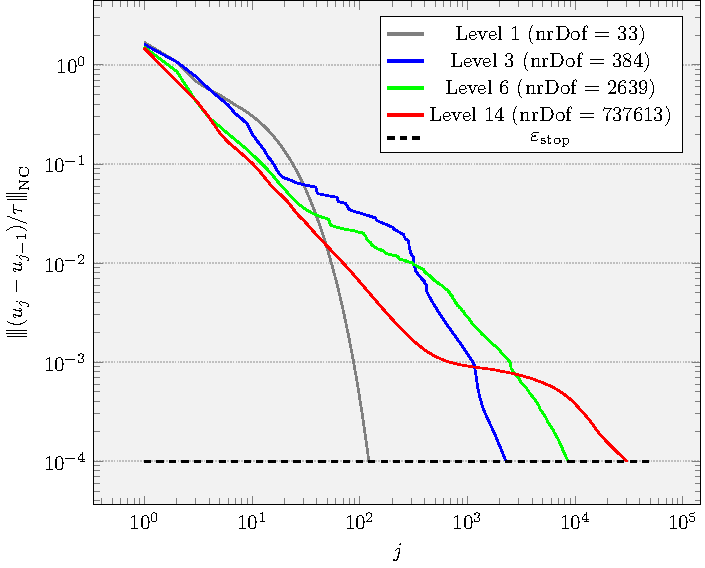
\includegraphics[width=\linewidth]
      {pictures/chapExperiments/secExactSol/iteration/lvlWise/termLvl.pdf}
    \label{fig:iterationLevel}
  \end{subfigure}
  \quad
  \begin{subfigure}[b]{.46\linewidth}
    \centering
    \caption{verschiedene mögliche Abbruchkriterien}
    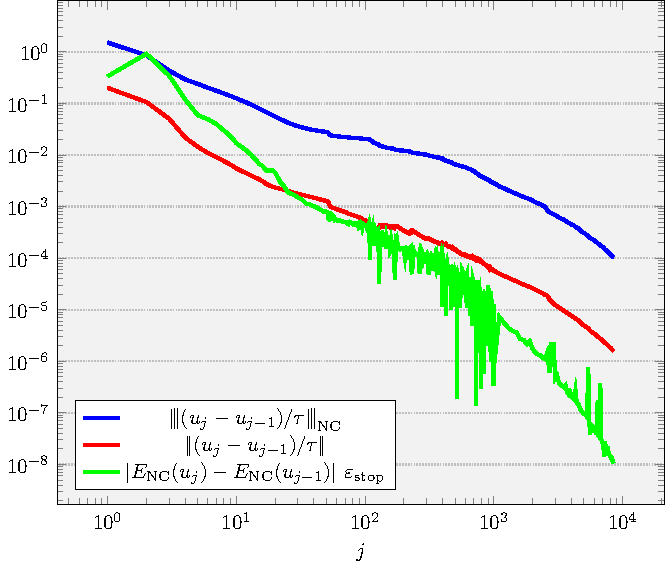
\includegraphics[width=\linewidth]
      {pictures/chapExperiments/secExactSol/iteration/lvlWise/termComp.pdf}
    \label{fig:iterationTerminationVariants}
  \end{subfigure}
  \caption{Abbruchkriterien wobei das initiale Level 0 ist.}
  \label{fig:iterationTermination}
\end{figure}

kleine tau und alpha nicht groß lässt die energie nur osszilierend von oben
konvergieren (s. Ordner) (auch tau = h/10 oder so ähnlich (bartels))
wird alpha zu kleinen tau groß gewählt, behebt dass den Effekt.


3) $|||.||| ~ h^{-1} ||.||$ korrekt? Enc stetig bzgl Konvergenz in L2 (Zsmh. 
   zwischen eNc und bar12sqrt)
   (discrete Poincare (bar15, Lem 3.7), inverse Ungleichung (bar15, Lem. 3.5)),
   Bsp. Lvl13 in $f01eps10^{-4}$ hat hMin ~ $10^{-3}$, Graphen sehen korrekt
   verschoben aus


1) terminatin Criteria Vergleich (f01Term und camTerm)
    - eNcAbsDiff wegen Oszillation ungeeignet (da das mal 'zu früh') die 
      Toleranz erreichen kann obwohl es noch nicht soweit ist
    - die anderen sind alle gleich gut, oder? ist die Höhe der Graphen relevant?
      (natürlich müsste man epsStop analog kleiner wählen, wenn man z.B. den
      parallel und niedrigeren bar15TerminationWithoutL2 wählt)


==================

Nun betrachten wir Konvergenzraten und überprüfen die Gültigkeit einiger in den
theoretischen Kapiteln dieser Arbeit getätigten Aussagen.
\begin{figure}[p]
  \centering
  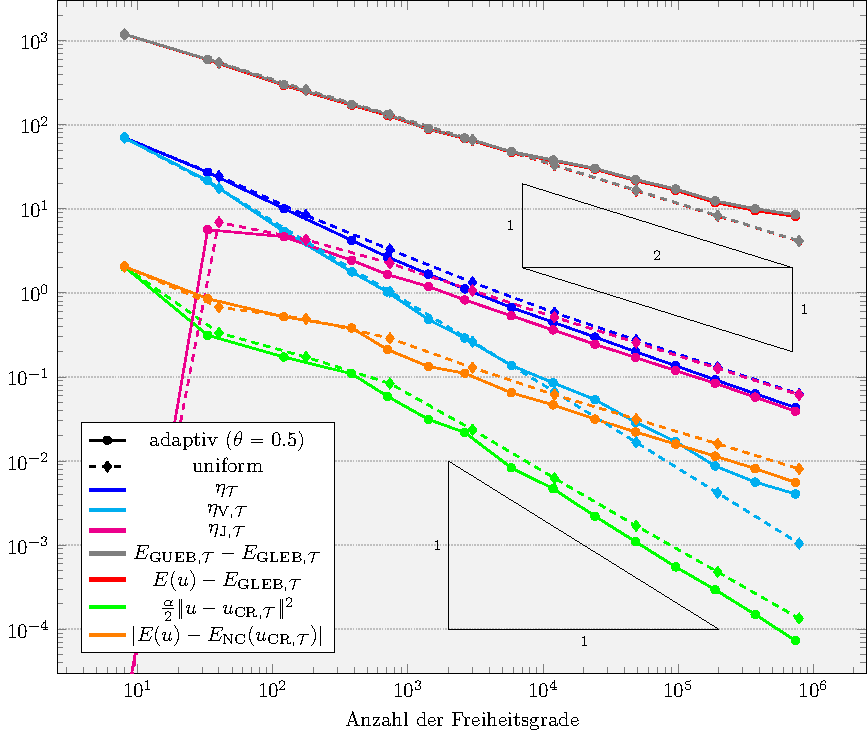
\includegraphics[width=\linewidth]
    {pictures/chapExperiments/secExactSol/f01/conv.pdf}
  \caption{Ergebnisse der adaptiven und uniformen AFEM-Schleifen für das 
  Eingangssignal $f$.}
  \label{fig:f01Convergence}
\end{figure}
\begin{figure}[p]
  \centering
  \begin{subfigure}[b]{.48\linewidth}
    \centering
    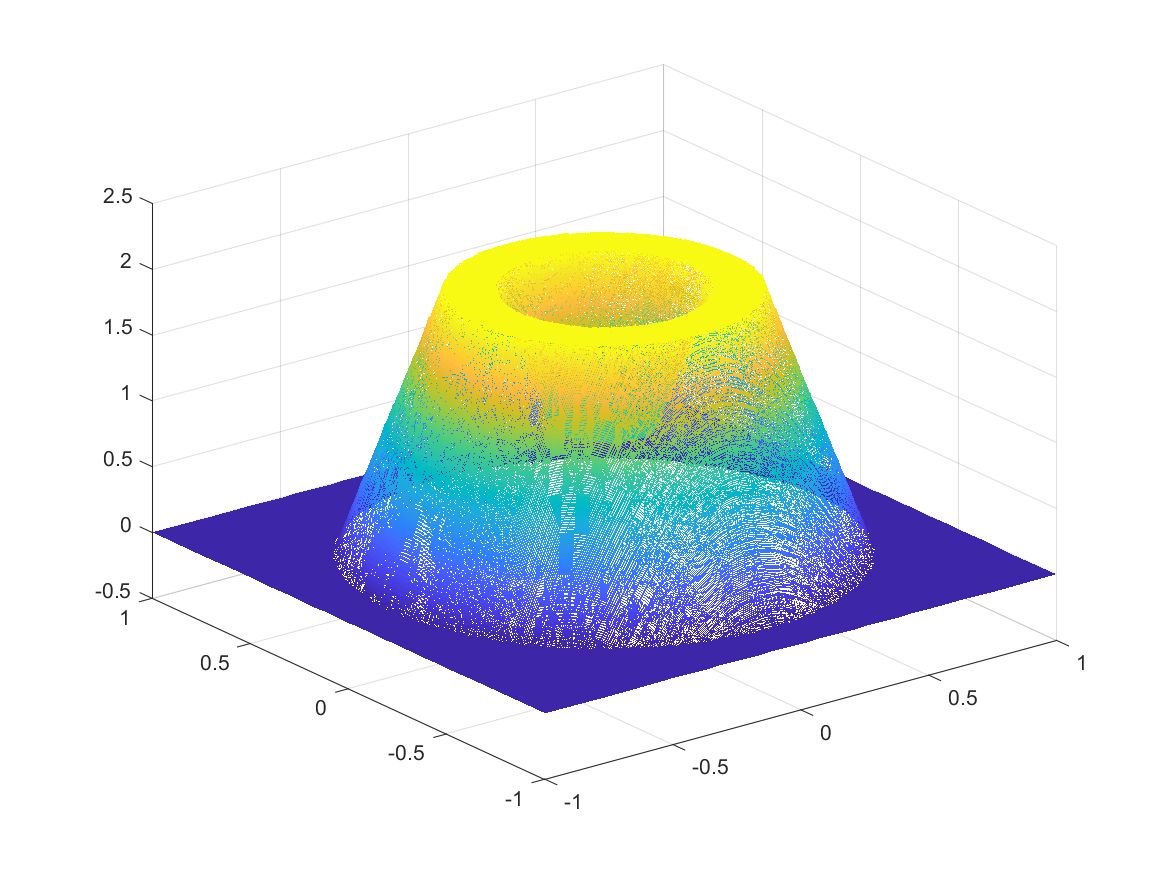
\includegraphics[trim = 40 30 30 30, clip, width=\linewidth]
      {pictures/chapExperiments/secExactSol/f01/adaptive/lvl14/solution.png}
    \label{fig:f01SolAdaptivePlot}
  \end{subfigure}
  \quad
  \begin{subfigure}[b]{.48\linewidth}
    \centering
    \includegraphics[trim = 50 30 50 20, clip, width=\linewidth]
      {pictures/chapExperiments/secExactSol/f01/adaptive/lvl14/solutionAxis.png}
    \label{fig:f01SolAdaptiveAxis}
  \end{subfigure}
  \caption{Lösung des adaptiven Algorithmus mit Eingangssignale $f$ sowie deren
  Darstellungen entlang der x-Achse (blau) und der y-Achse (rot).}
  \label{fig:f01SolAdaptive}
\end{figure}
\begin{figure}[p]
  \centering
  \begin{subfigure}[b]{.48\linewidth}
    \centering
    \caption{Unterschiede oberer beiden Graphen}
    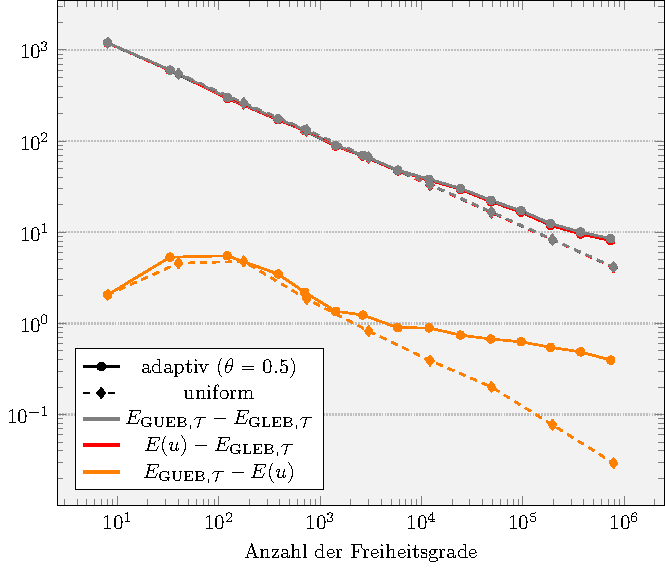
\includegraphics[width=\linewidth]
      {pictures/chapExperiments/secExactSol/f01/energyDiffs.pdf}
    \label{fig:f01DiffGuebExactE}
  \end{subfigure}
  \quad
  \begin{subfigure}[b]{.48\linewidth}
    \centering
    \caption{Sprungterm Entwicklung}
    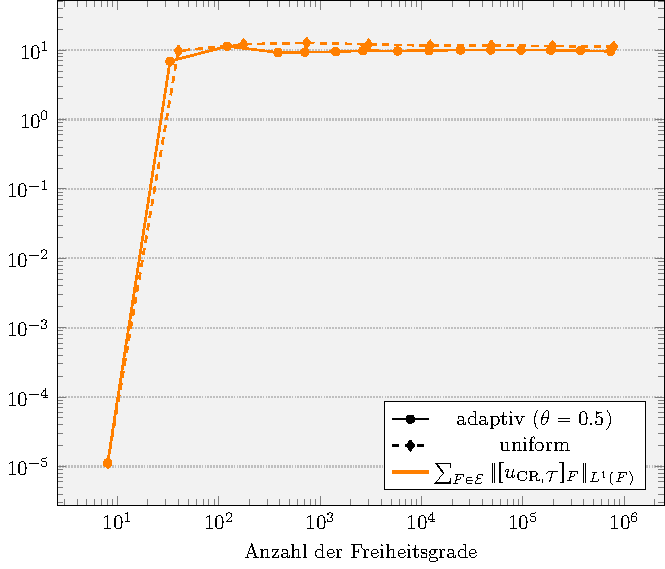
\includegraphics[width=\linewidth]
      {pictures/chapExperiments/secExactSol/f01/jumpTerms.pdf}
    \label{fig:f01JumpTerms}
  \end{subfigure}
  \caption{Zusätzliche Infos für Eingangangssignal $f$.}
  \label{fig:f01SupplementaryInfo}
\end{figure}
Wie in \Cref{fig:f01Convergence} zu sehen, unterscheiden sich die Raten für
uniforme und adaptive Netzverfeinerungen nicht.

Es gilt 
\begin{align}
  \label{eq:expectedInequalities}
  \frac{\alpha}{2}\Vert u -\ucrt\Vert^2
  \leq
  E(u)-\Egleb
  \leq
  \Egueb-\Egleb,
\end{align}
wie wir nach \Cref{thm:gleb} und Ungleichung \ref{eq:gueb} erwartet haben.
Dabei merken wir an, dass dieser Sachverhalt für $E(u)-\Egleb\leq\Egueb-\Egleb$
nur schwer zu erkennen ist, aber gilt, wie dank \Cref{fig:f01DiffGuebExactE} zu
sehen ist, da $\Egueb-\Egleb-(E(u)-\Egleb) = \Egueb-E(u)$.
In \Cref{fig:f01JumpTerms} sehen wir weiterhin, dass die Sprungterme in
unserere nichtkonformen Formulierung tatsächlich nicht minimiert werden. 
Zwar sind die jeweiligen Sprünge zwischen zwei Dreiecken bei einer hohen Anzahl
von Freiheitsgraden klei, wie \Cref{fig:f01SolAdaptive} erahnen lässt, jedoch
wird durch die hohe Anzahl von Kanten ein große Menge von kleinen Sprüngen
addiert, die zu einer relativ großen Summe führen.
Da durch \Cref{fig:f01Convergence} zu sehen ist, dass $|E(u)-\Enc(\ucrt)|$
konvergiert, wird klar, dass $E(\ucrt)$ nicht gegen $E(u)$ konvergiert, wie zu
erwarten war nach \Cref{sec:discreteProblemFormulation}.
Zudem lässt sich die Konvergenz von $\Enc(\ucrt)$ gegen $E(u)$ durch betrachten
von \Cref{fig:iterationEnergyLevel} erahnen, in der der Abstand des 
augenscheinlichen Grenzwerts der Iteration mit höhrerem Level näher an $E(u)$
liegt.
Aus \Cref{thm:convexity} und \Cref{sec:discreteProblemFormulation} folgt
\begin{align*}
  \frac{\alpha}{2}\Vert u-\ucrt\Vert^2\leq
  E(\ucrt)-E(u)=\Enc(\ucrt)+\sum_{F\in\Ecal}\Vert[\ucrt]_F\Vert_{L^1(F)}-E(u).
\end{align*}
Insbesondere gilt auch 
\begin{align*}
  \frac{\alpha}{2}\Vert u-\ucrt\Vert^2
  \leq
  \left|\Enc(\ucrt)-E(u)\right|+
  \sum_{F\in\Ecal}\Vert[\ucrt]_F\Vert_{L^1(F)}.
\end{align*}
Dieser Aussage widerspricht \Cref{fig:f01Convergence} nicht, obwohl die Sprünge,
die auf der rechten Seite dieser Ungleichung stehen, im Plot nicht einbezogen
sind.


==================

dann insgesamt raten abarbeiten und interpretieren

==================

\begin{figure}[p]
  \centering
  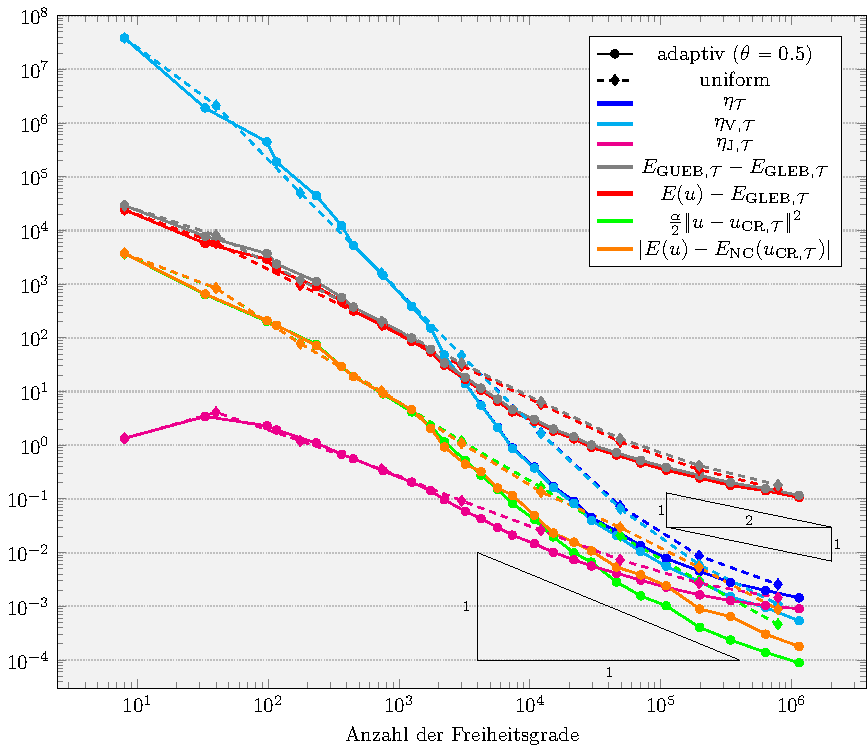
\includegraphics[width=\linewidth]
    {pictures/chapExperiments/secExactSol/f01LargeAlpha/conv.pdf}
  \caption{Ergebnisse der adaptiven und uniformen AFEM-Schleifen für das 
  Eingangssignal $f$ mit $\alpha=10^4$.}
  \label{fig:f01LargeAlphaConvergence}
\end{figure}

  - f01 mit großem alpha konvergiert am Anfang preasymptotisch schnell aber
    scheint bei großen Freiheitsgraden dann auch die Rate 1/2 (für Gleb Kram)
    bzw. 1/4 oder so für Fehler anzunehmen (also gleiche Raten wie alpha=1).
    liegt daran, dass für große alpha die Werte anfangs explodieren und damit
    die Konvergenz rapide ist (auch die Iterationen sind viel kürzer, hier
    lohnt sich sicherlich auch der Vergleich der misc plots und nochmal verweis
    auf die Abschätzung aus Konvergenzbeweis (großes alpha, womöglich weniger
    Iteration))

    Zum Plot der rechten Seite $f_\textup{L}$ kann man sagen, dass man hier die
    Theorie der ROF Modells sieht, da für dieses große $\alpha$ ja zu erwarten
    ist nach der Theorie, dass die Lösung $u_\textup{L}$ und
    $f_\textup{L}=\alpha g$ nahe beiandere liegen, was sie tatsächlich 
    optisch auch tun

Es scheint bei alpha groß so, dass die einzige Rate, die sich am Ende 
unterscheidet, die Energiedifferenz ist (die konvergiert fur großes
alpha nämlich mit 1 und nicht mit 1/2 wie bei alpha =1)

Wir bemerken, dass das Eingangssignal so aussieht, wie $\alpha u$ mit $u$ aus
\Cref{fig:f01ExactSol}. Dies war nach der Theorie auch \Cref{chap:introduction}
so zu erwarten.

Wir sehen auch annähernd den erwarten Unterschied $h_T$ zwischen den Differenzen
in der $L^2$-Norm und der Norm $\vvvert\bullet\vvvert_\NC$, wobei hier
$h_T=\sqrt{2}$, $h_\text{min}=1$.
Das eintreten dieser erwarteten Unterschiede (Erläuterung der 
Skalierugsunterschiede im Beweis von Lemma \ldots (Stetigkeit vor
Minimierer Beweis))
==================

\begin{figure}[p]
  \centering
  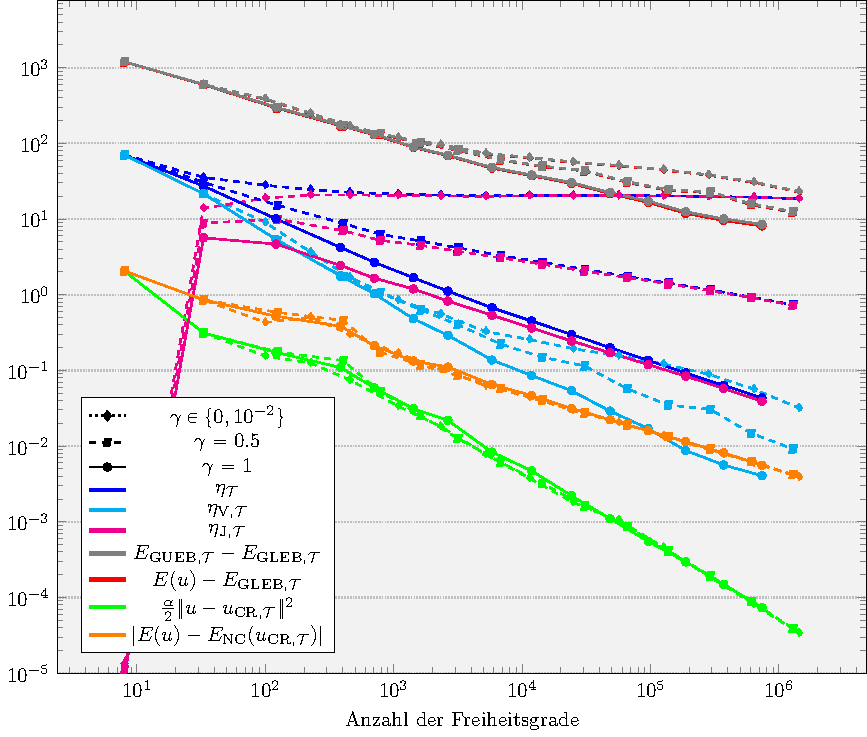
\includegraphics[width=\linewidth]
    {pictures/chapExperiments/secExactSol/parGamma/conv.pdf}
  \caption{$\gamma$ Plots.}
  \label{fig:parGammaConvergence}
\end{figure}

\begin{figure}[p]
  \centering
  \begin{subfigure}{.32\linewidth}
    \centering
    \caption{$\gamma=0$}
    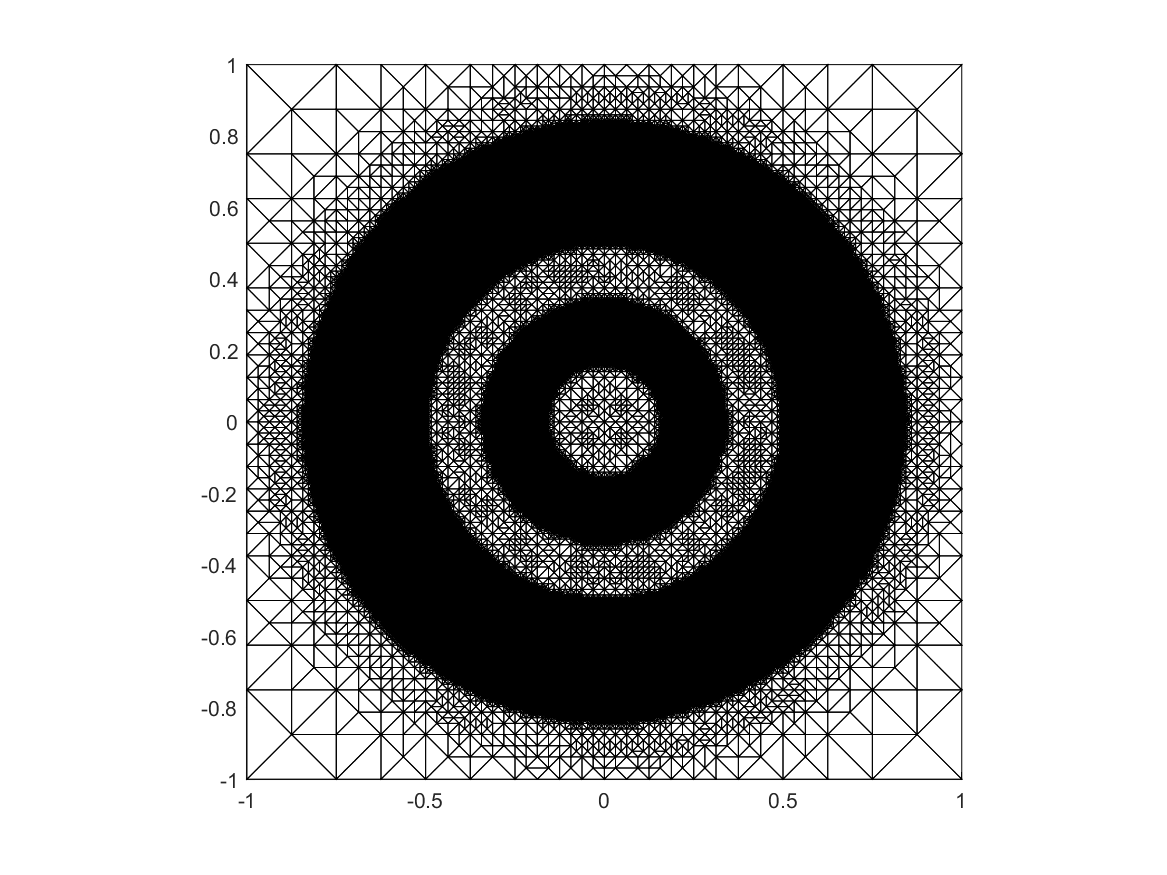
\includegraphics[trim = 100 30 80 20, clip, width=\linewidth]
      {pictures/chapExperiments/secExactSol/parGamma/0/lvl14/triangulation.png}
    \label{fig:gamma0Triang}
  \end{subfigure}
  \begin{subfigure}{.32\linewidth}
    \centering
    \caption{$\gamma=0.5$}
    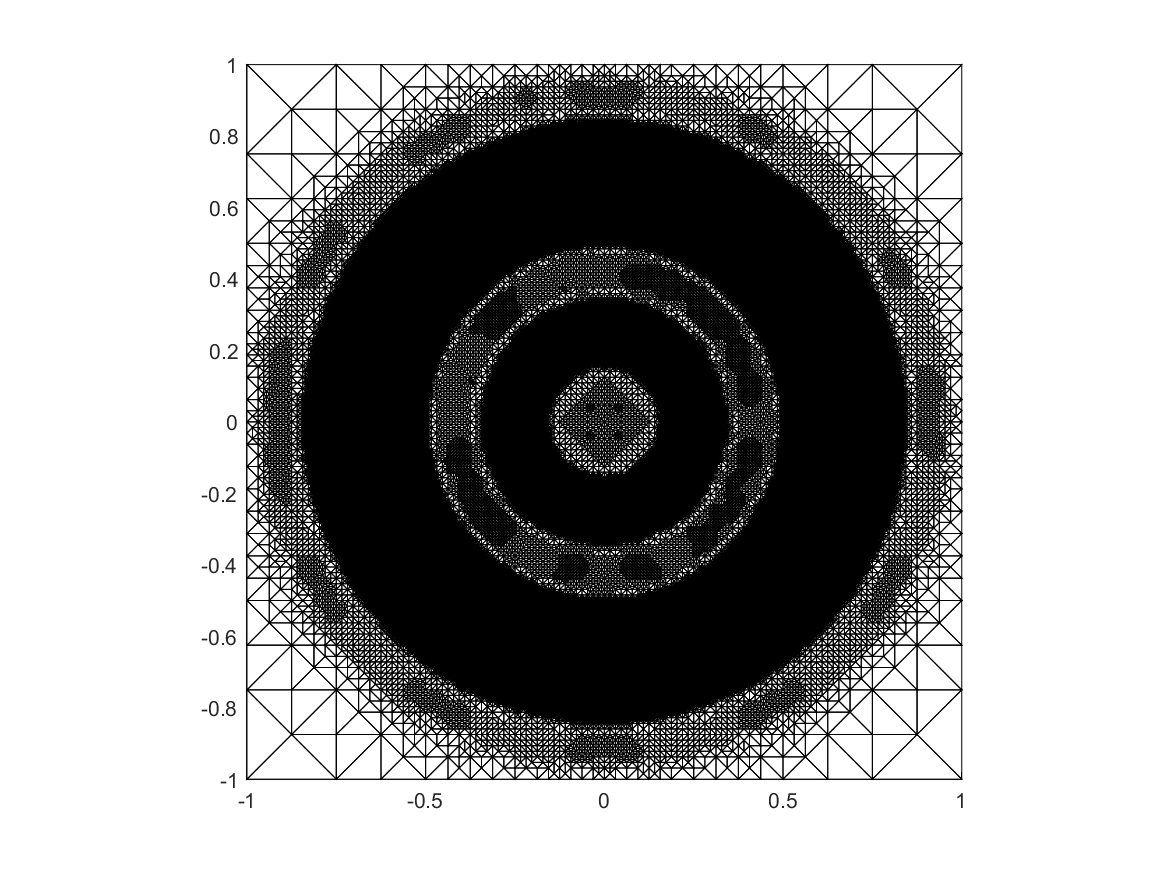
\includegraphics[trim = 100 30 80 20, clip, width=\linewidth]
      {pictures/chapExperiments/secExactSol/parGamma/5em1/lvl14/triangulation.png}
    \label{fig:gammaDot5Triang}
  \end{subfigure}
  \begin{subfigure}{.32\linewidth}
    \centering
    \caption{$\gamma=1$}
    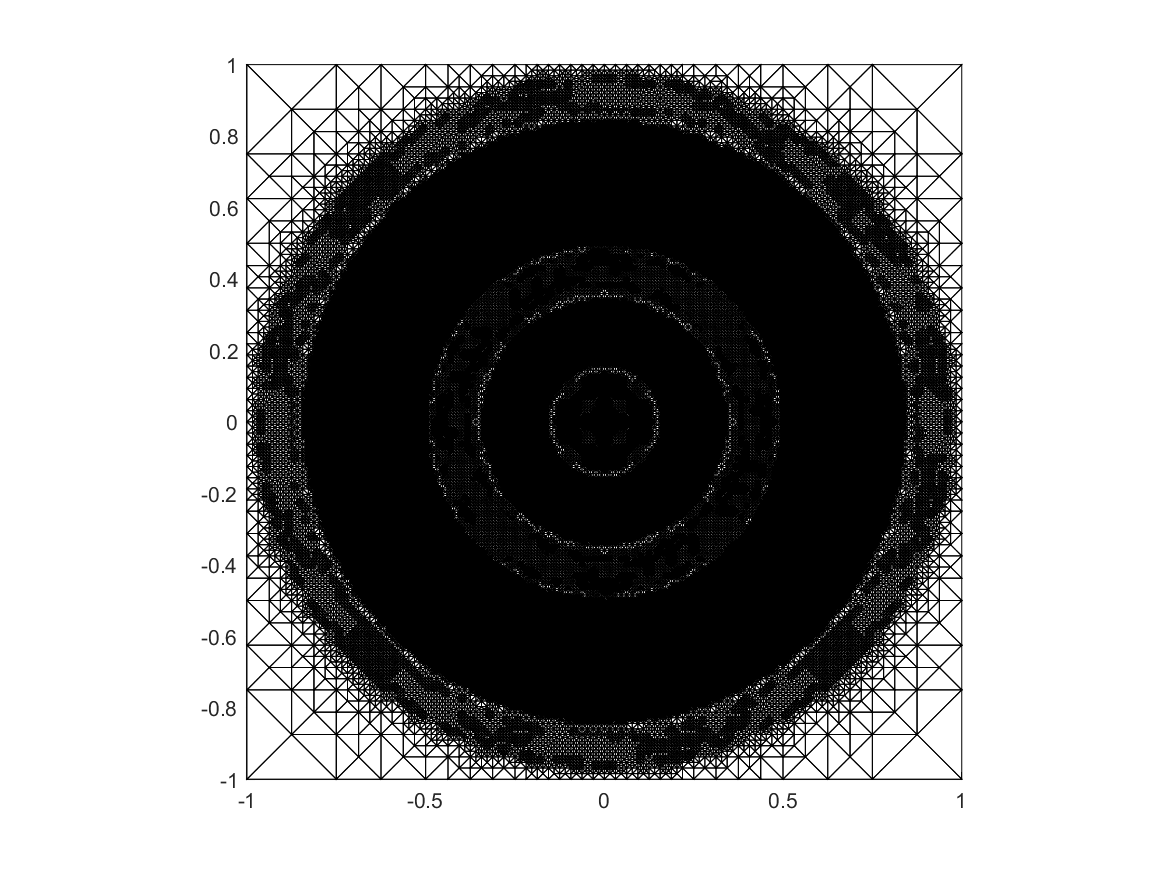
\includegraphics[trim = 100 30 80 20, clip, width=\linewidth]
      {pictures/chapExperiments/secExactSol/parGamma/1/lvl14/triangulation.png}
    \label{fig:gamma1Triang}
  \end{subfigure}
  \caption{$\gamma$ Triangulierungen Plots.}
  \label{fig:gammaTriangs}
\end{figure}
zu gamma (0, 0.5, 1) noch irgendwo ein Experiment mit Info, dass 0 und 1e-4 oder
so was identisch sind

  - gamma = 0 im Vergleich der gammas mit erwähnen (da es sich von gamma 1e-2
    nicht unterscheider visuell nur eines der

    die Plots für gamma = 1 entsprechen natürlich exact den Graphen aus
    \Cref{fig:f01Convergence}

    wir können den Effekt auch in den Triangulierungen (vlt jeweils noch die
    nrDof auslesen lassen) aus \Cref{fig:gammaTriangs} sehen

drüber nachdenken, ob hier gamma größe nochmal angeguckt werden könnte bei
cont circle (vlt auch einfach nicht, ging ja nur um die allgemeine wahl für
gamma, um eine entscheidung zu treffen, zuvor)

das vielleicht auch doch erst im nächsten Abschnitt nachdem schon gesehen wurde,
dass Raten für adaptiv und uniform gleich sind (da das der Fall ist, ist mit 
'noch stärkerer' adaptivität keine Verbesserung mehr zu erwarten (suche das 
Blatt, wo diese Worte von Tien drauf stehen)) 

stärkere adaptivität heißt, dass wir mit kleinerem $\gamma$ krasser 
zu den Sprüngen hin verfeinern, was kontraproduktiv ist, wohl auch, da wir
Sprünge ja garnicht mehr minimieren in unserem Funktional

In der Abbildung ist tatsächlich $\gamma= 10^{-2}$ nicht abgebildet, da
die entsprechend Graphen sich nicht sichtbar vom Graphen für $\gamma=0$
unterschieden haben.

\Cref{eq:expectedInequalities} ist aber auch hier weiterhin gültig, was gut 
ist

mal gucken,die Sprungterme oder irgendwas stehen auch im Gleb oder sowas, 
damit also wohl mal versuchen zu erklären, warum manche Graphen beinflusst
werden und andere nicht

insgesamt nochmal den Verfeinerungsindikator analysieren und sagen,
was da für die kleineren Werte passiert

hier dann endlich ein beispiel, bei dem adaptivität besser ist, (sowohl
etaJ als auch etaV, was sogar erwartbar ist, da es hier eine so klare 
antwort gibt, wo man verfeinern möchte und wo nicht und das sieht man dann
auch in den raten, die wären \ldots)

das sich zwischen steig und unsteig nur der gueb-gleb graph unterscheidet 
wird schlicht und ergreifend daran liegen, dass es die gleb aussage
für unsteig (da nicht h10) nicht gibt und das nur berechnet wird, weil es halt 
geht
alles, was es für beide wirklich gibt (unklar, vlt nicht sagen,
Verfeinerungsindikator folgt ja immer auch gleb oder sowas) ist gleich

==================

hier eventuell auch experimte für AFEM Params? die werden am anfang mit
,stets, wenn nicht anders angegeben' deklariert und hier wird experementiert

==================

  Es folgt ein Beispiel mit exakter Lösung $u_\textrm{HR} \in
  H^2_0((0,1)^2)$, gegeben durch 
\begin{align*}
  u_\textrm{HR}(r)\coloneqq 
  \begin{cases}
    1, & \text{wenn } 0\leq r\leq\frac{1}{3},\\
    54r^3 - 81r^2 + 36r - 4, & 
    \text{wenn } \frac{1}{3}\leq r\leq \frac{2}{3},\\
    0, & \text{wenn } \frac{2}{3}\leq r.
  \end{cases}
\end{align*}
Mit der Wahl
\begin{align*}
  \sgn&(\partial_r u_\textrm{HR}(r)) \\
  &\coloneqq 
  \begin{cases}
    -1458r^5 + 1215r^4 - 270r^3, & \text{wenn } 0\leq r\leq\frac{1}{3},\\
    -1, & \text{wenn } \frac{1}{3}\leq r\leq \frac{2}{3},\\
    -243r^4 + 756r^3 - 864r^2 + 432r - 81, 
    & \text{wenn } \frac{2}{3}\leq r\leq 1,
  \end{cases}
\end{align*}
erhalten wir die rechte Seite
\begin{align*}
  f_\textrm{HR}(r)\coloneqq 
  \begin{cases}
    \alpha + 8748r^4 - 6075r^3 + 1080r^2, &
    \text{wenn } 0\leq r\leq\frac{1}{3},\\
    \alpha\left(54r^3 - 81r^2 + 36r - 4\right) + \frac{1}{r}, & 
    \text{wenn } \frac{1}{3}\leq r\leq \frac{2}{3},\\
    1215r^3 - 3024r^2 + 2592r - 864 + \frac{81}{r}, & 
    \text{wenn } \frac{2}{3}\leq r\leq 1,
  \end{cases}
\end{align*}
für die gilt $f_\textrm{HR}\in H^2_0$.


\begin{align*}
  \partial_r f_\textrm{HR}(r) &=
  \begin{cases}
    34992r^3 - 18225r^2 + 2160r, & \text{wenn } 0\leq r\leq\frac{1}{3},\\
    \alpha\left(162r^2 - 162r + 36\right) - \frac{1}{r^2}, & 
    \text{wenn } \frac{1}{3}\leq r\leq \frac{2}{3},\\
    3645r^2 - 6048r + 2592 - 864 - \frac{81}{r^2}, & 
    \text{wenn } \frac{2}{3}\leq r\leq 1,
  \end{cases}
\end{align*}
\begin{align*}
  \partial_r u_\textrm{HR}(r) &=
  \begin{cases}
    0, & \text{wenn } 0\leq r\leq\frac{1}{3},\\
    162r^2 - 162r + 36, & 
    \text{wenn } \frac{1}{3}\leq r\leq \frac{2}{3},\\
    0, & \text{wenn } \frac{2}{3}\leq r\leq 1,
  \end{cases}
\end{align*}

\begin{figure}[p]
  \centering
  \begin{subfigure}[b]{.48\linewidth}
    \centering
    \caption{$f_\textrm{HR}$}
    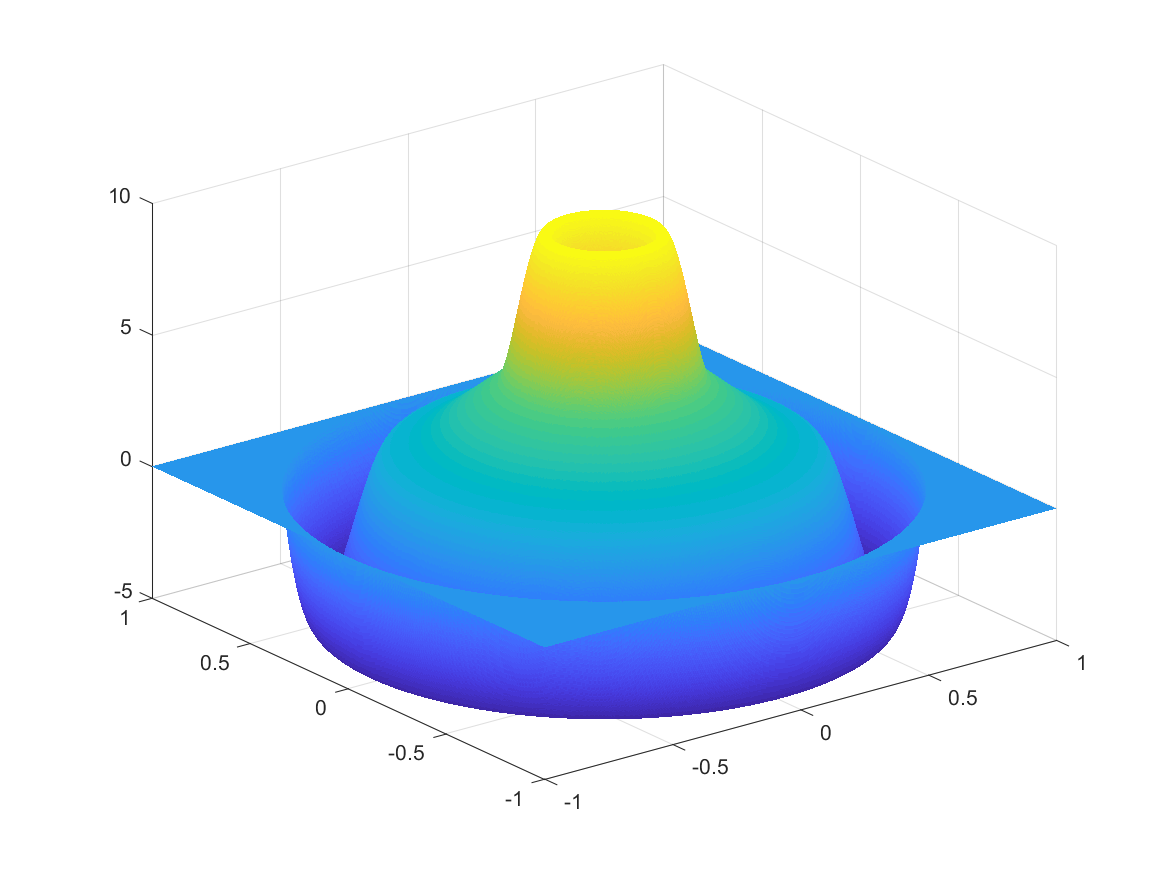
\includegraphics[trim = 40 30 30 30, clip, width=\linewidth]
      {pictures/chapExperiments/secExactSol/f04/inSi.png}
    \label{fig:f04InSi}
  \end{subfigure}
  \quad
  \begin{subfigure}[b]{.48\linewidth}
    \centering
    \caption{$f_\textrm{HR}$ entlang der x- und y-Achse}
    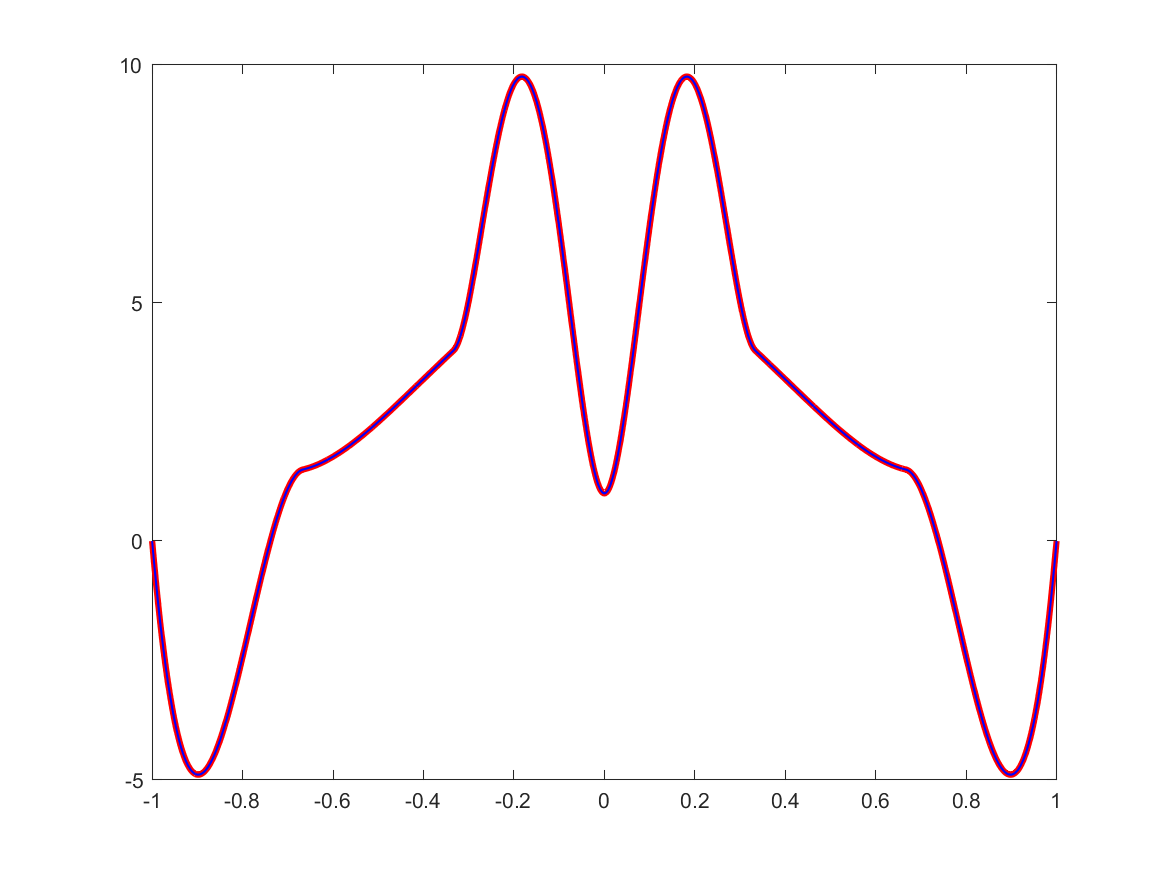
\includegraphics[trim = 50 30 50 20, clip, width=\linewidth]
      {pictures/chapExperiments/secExactSol/f04/inSiAxis.png}
    \label{fig:f04InSiAxis}
  \end{subfigure}

  \begin{subfigure}[b]{.48\linewidth}
    \centering
    \caption{$u_\textrm{HR}$}
    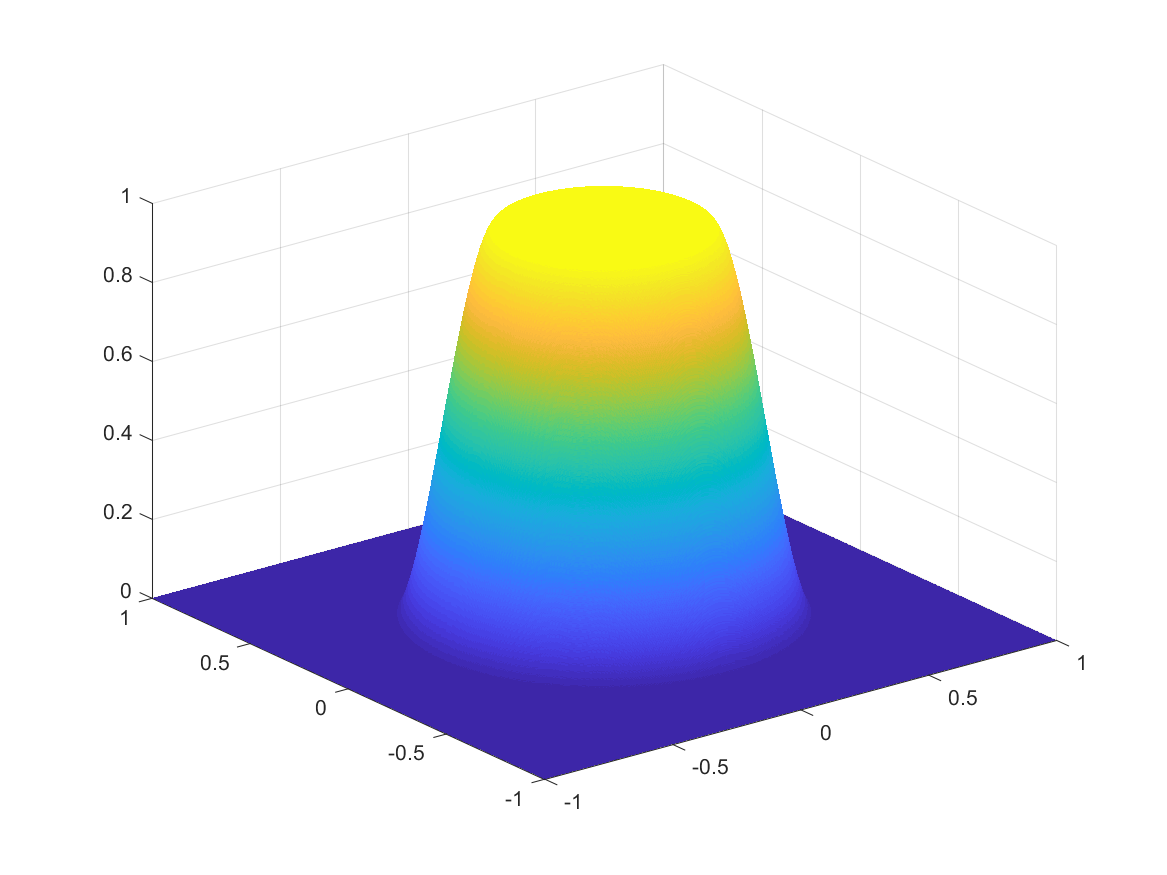
\includegraphics[trim = 40 30 30 30, clip, width=\linewidth]
      {pictures/chapExperiments/secExactSol/f04/exactSolution.png}
    \label{fig:f04ExactSol}
  \end{subfigure}
  \quad
  \begin{subfigure}[b]{.48\linewidth}
    \centering
    \caption{$u_\textrm{HR}$ entlang der x- und y-Achse}
    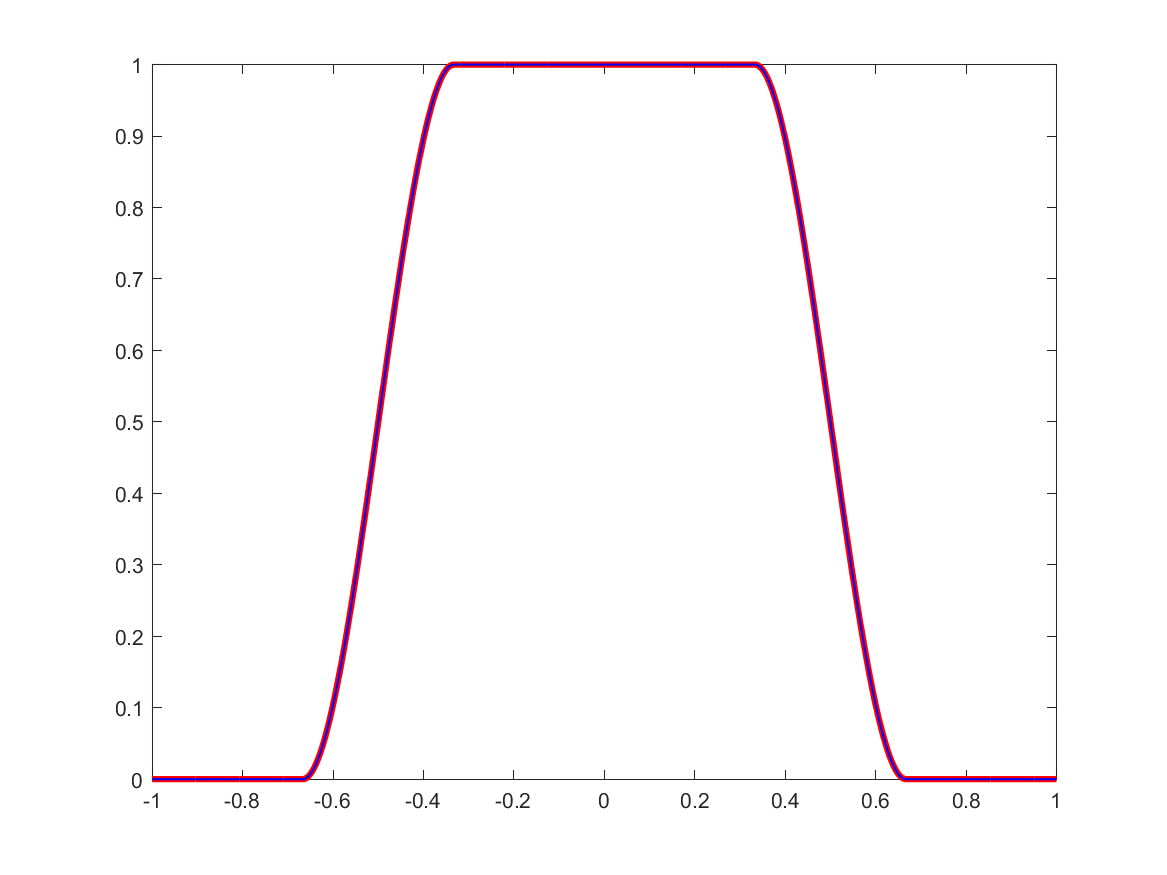
\includegraphics[trim = 50 30 50 20, clip, width=\linewidth]
      {pictures/chapExperiments/secExactSol/f04/exactSolutionAxis.png}
    \label{fig:f04ExactSolAxis}
  \end{subfigure} 
  \caption{Eingangssignal $f_\textrm{HR}$ und exakte Lösung $u_\textrm{HR}$
  sowie deren Darstellungen entlang der x-Achse (blau) und der y-Achse (rot)
  für $\alpha=1$.}
  \label{fig:f04Plots}
\end{figure}
\begin{figure}[p]
  \centering
  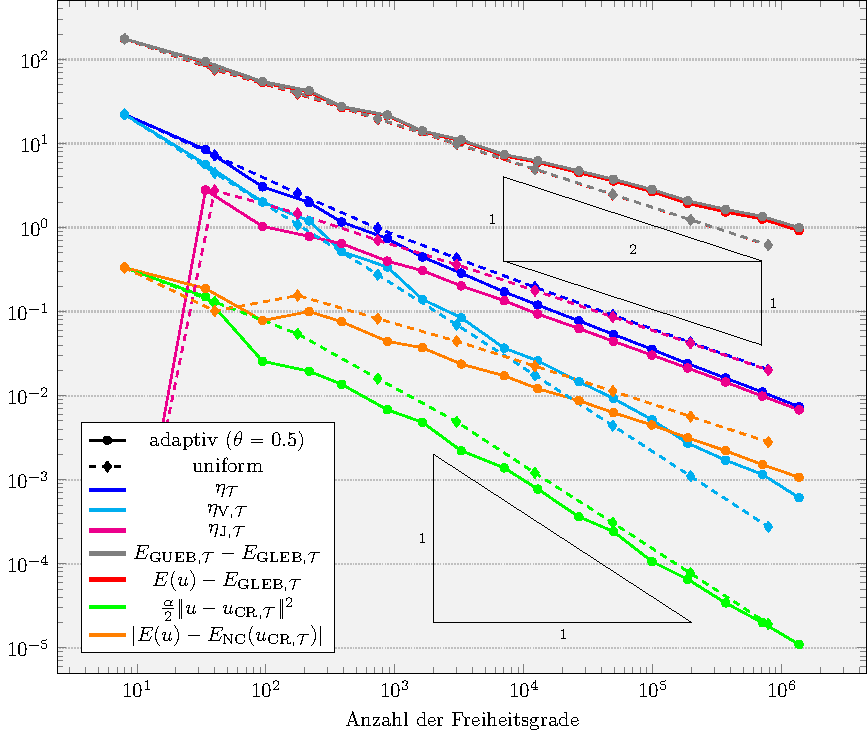
\includegraphics[width=\linewidth]
    {pictures/chapExperiments/secExactSol/f04/conv.pdf}
  \caption{Ergebnisse der adaptiven und uniformen AFEM-Schleifen für das 
  Eingangssignal $f_\textrm{HR}$.}
  \label{fig:f04Convergence}
\end{figure}

dann abschweif zu höhere Regularität

  hier kann vlt auch nochmal auf die Abschätzung mit der $\tau$ begründet wurde
  eingegangen werden (zwar führt alpha zu einem anderen Experiment, aber 
  trotzdem kann festgestellt werden, dass hier weniger Iterationen als für
  $\alpha=1$ benötigt wurden), d.h. Verweis auf vorherige section

  wir sehen deutlich bessere Raten als in Bartels flg. Thm. :

  folgendes wird definitiv erwähnt werden, zumindest das Resultat, und dabei
  wird nochmal $S^1(\Tcal)$ notiert werden

  Zunächst betrachten wir \cite[S. 309, Theorem 10.7]{Bar15}. Diese
  Abschätzung kontrolliert den
  $L^2$-Fehler zwischen den Minimierern $u_\C\in S^1(\Tcal)$ und
  $u\in\BV(\Omega)\cap L^2(\Omega)$ des Funktionals $I$ aus \Cref{eq:rofModel} in
  den entsprechenden Räumen. Obwohl wir eine andere Formulierung des ROF-Modells 
  betrachten und sich insbesondere das Funktional $\Enc$ aus unserer diskreten,
  nichtkonformen Formulierung von $I$ unterscheidet, ähneln sich die 
  Probleme möglicherweise genug, um die folgende Rate für unsere Formulierungen
  experimentell feststellen zu können.
  
  \begin{theorem}
    \label{thm:errorEstimateCourant}
    Sei $\Omega\subset\Rbb^2$ sternförmig und $g\in L^\infty(\Omega)$.  Seien
    weiterhin $u\in\BV(\Omega)\cap L^2(\Omega)$ und $u_\C\in S^1(\Tcal)$ die
    Minimierer des Funktionals $I$ aus \Cref{eq:rofModel} in den entsprechenden
    Räumen.
  
    Dann existiert eine Konstante $c\in\Rbb_+$, sodass
    \begin{align*}
      \frac{\alpha}{2}\Vert u-u_\C\Vert^2\leq
      ch^{1/2}.
    \end{align*}
  \end{theorem}

  da wir hohe Regularität haben mit H10, d.h. höher als im Thm angenommen, ist
  dies zu erwarten. Ein kurzes Experiment soll untersuchen, ob noch höhere 
  Reg.annahmen die Raten weiter verbessern
  - h20 Beispeil genau so wie H10, also das vielleicht nur erwähnen ,,eine 
    noch stärke Regularitätsannahme im Beispeil f04, bei dem Lsg und f H20 sind,
    verbesserte die Raten nicht weiter (verschiebt nur die Graphen nach unter,
    d.h. früher kleiner Fehler)

  nur halb H20 Beispiel auch erwähnen, einfach sagen, dass dieses auch im 
  functions Ordner liegt

  
==================

\begin{figure}[p]
  \centering
  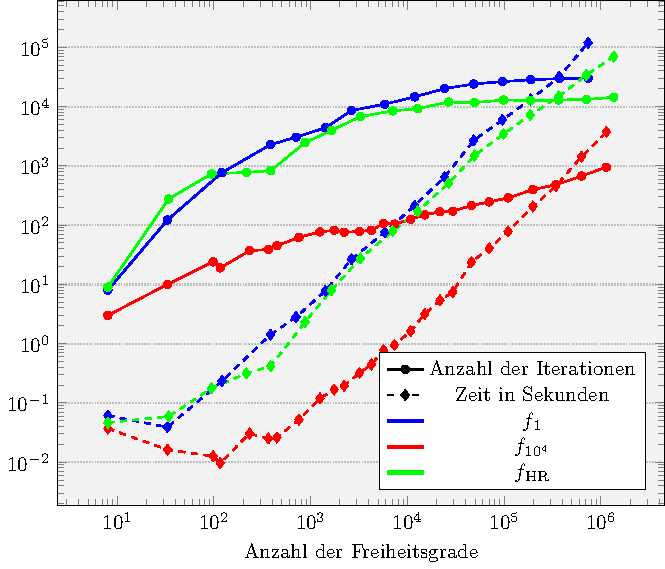
\includegraphics[width=\linewidth]
    {pictures/chapExperiments/secExactSol/nrIterComp/miscF.pdf}
  \caption{Vergleich der Iterationen fur verschiedene Eingangssignale.}
  \label{fig:inSiNrIterComparison}
\end{figure}

plot in der anzahl der iteration verglichen werden für f01,
f01LargeAlpha und f04 (natürlich alle mit $\tau=1$, weil  f01LargeAlpha die
wenigsten Iteration braucht (obwohl ähnlich
zu f01 (insb. gleiche Lösung) und obwohl f04 regulärer). 
das kann dann wieder
mit der erwarteten Ungleichung aus dem Konvergenzbeweis begründet werden (also
sagen, dass man hier ein weiteres Indiz für diese Hypothese hat.
Noch drüber nachdenken: warum machen sachen mit alpah groß mehr Level im AFEM
Alg?


\section{Graufarbenbilder als Eingangssignale}
\label{sec:grayscalePicturesAsInputSignal}

In diesem Abschnitt wollen wir nun auch Beispiele untersuchen, bei denen
der schwache Gradient des Eingangssignals sowie die exakte Lösung nicht bekannt
sind und prüfen, welche Aussagen wir für diese treffen können.
Unser Hauptaugenmerk liegt auf dem Eingangssignal \texttt{cameraman} aus
\Cref{fig:cameraman}. 
Insbesondere können wir an diesen Beispielen gut veranschaulichen, wie
der Verfeinerungsindikator wirkt.

==================
cameraman 

\begin{figure}[p]
  \centering
  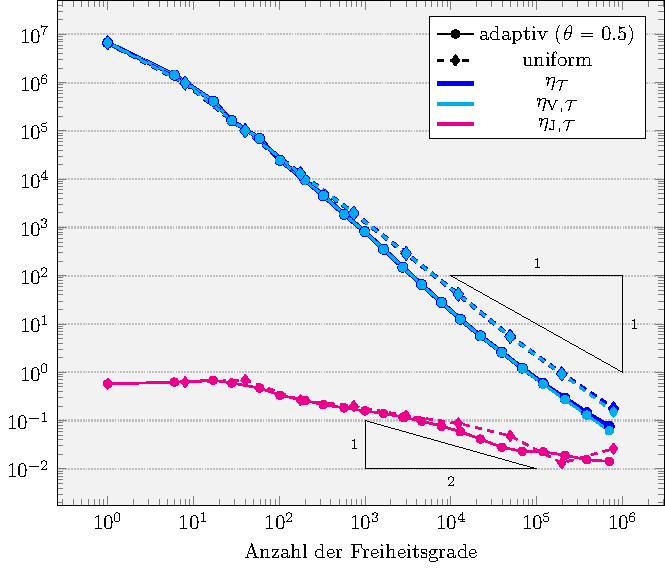
\includegraphics[width=\linewidth]
    {pictures/chapExperiments/secGrayscale/cam/conv.pdf}
  \caption{Ergebnisse der adaptiven und uniformen AFEM-Schleifen für das 
  Eingangssignal \texttt{cameraman}.}
  \label{fig:camConvergence}
\end{figure}

konvergenzplot adptiv/uniform
hier vielleicht gueb-Enc(ucr) plotten, mit dem Kommentar, dass dies uU
eine gute approximation von gueb - E(u) = gueb-gleb-(E(u)-gleb) ist, da 
wir in allen anderen experimten die konvergenz von Enc(ucr) gegen E(u) gesehen
haben und in dem einen plot von f01, in dem gueb - E(u) geplottet war,
 waren die raten entsprechend gleich (?)

für lvl 17 auf jeden fall nebenbeinander triangulierg | lösung auf der triang

\begin{figure}[p]
  \centering
  \begin{subfigure}[b]{.48\linewidth}
    \centering
    \caption{Triangulierung Level 17}
    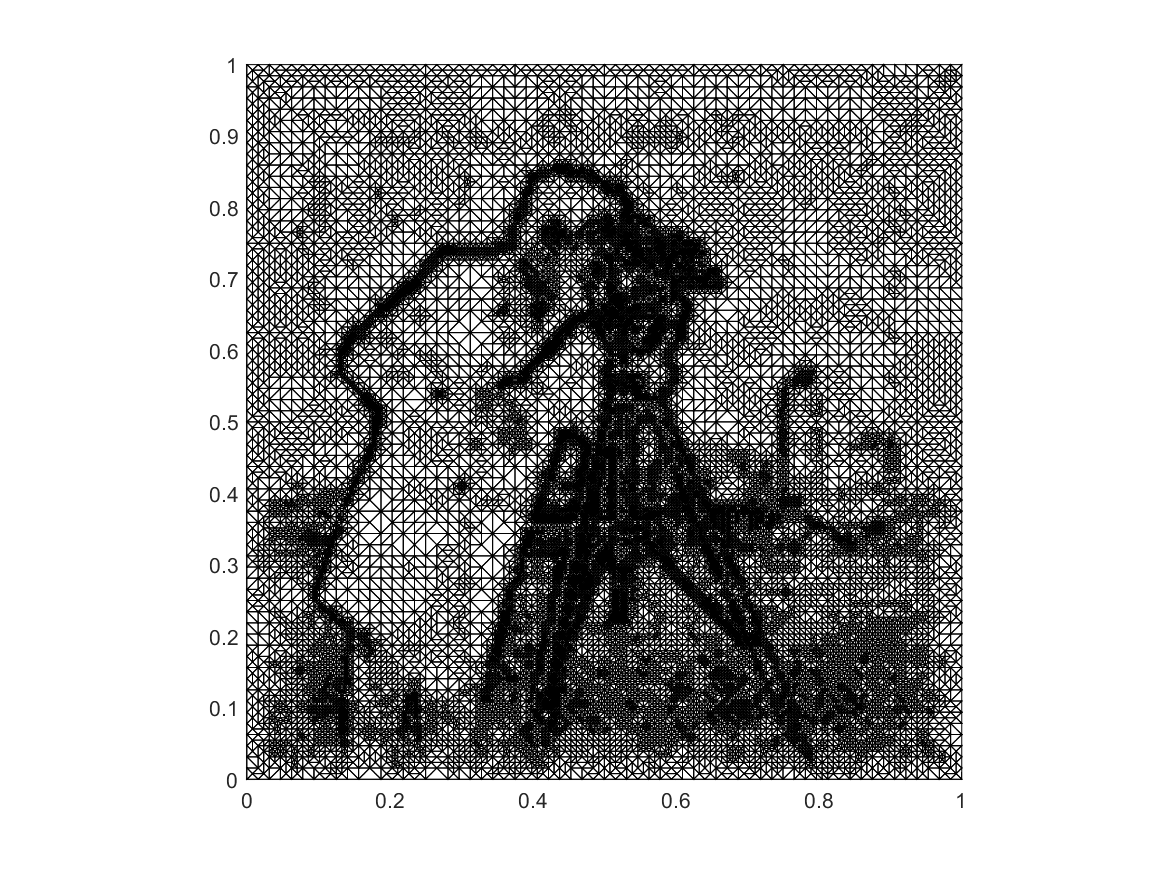
\includegraphics[trim = 100 30 80 20, clip, width=\linewidth]
      {pictures/chapExperiments/secGrayscale/cam/adaptive/lvl17/triangulation.png}
    \label{fig:camLvl17Triang}
  \end{subfigure}
  \quad
  \begin{subfigure}[b]{.48\linewidth}
    \centering
    \caption{Lösung Level 17}
    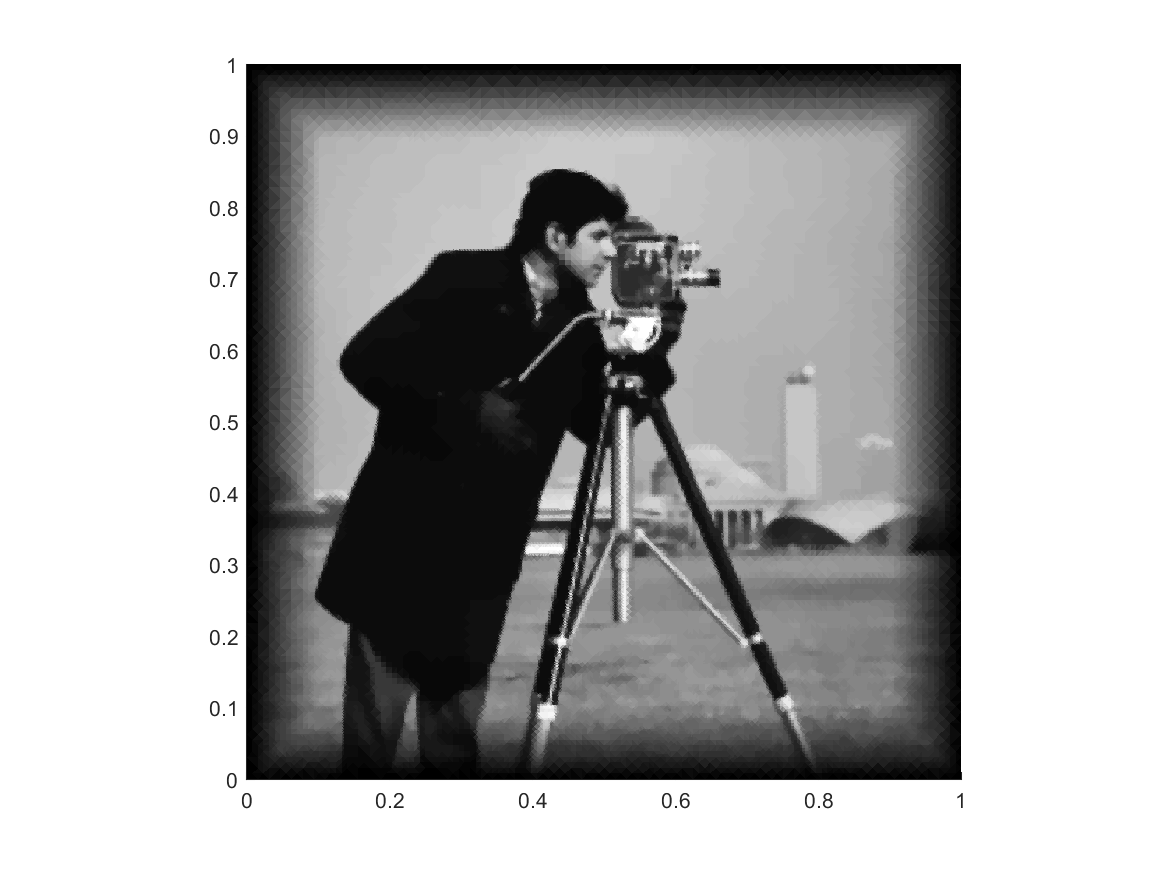
\includegraphics[trim = 100 30 80 20, clip, width=\linewidth]
      {pictures/chapExperiments/secGrayscale/cam/adaptive/lvl17/solutionGrayscale.png}
    \label{fig:camLvl17Sol}
  \end{subfigure}

  \begin{subfigure}[b]{.48\linewidth}
    \centering
    \caption{Triangulierung Level 21}
    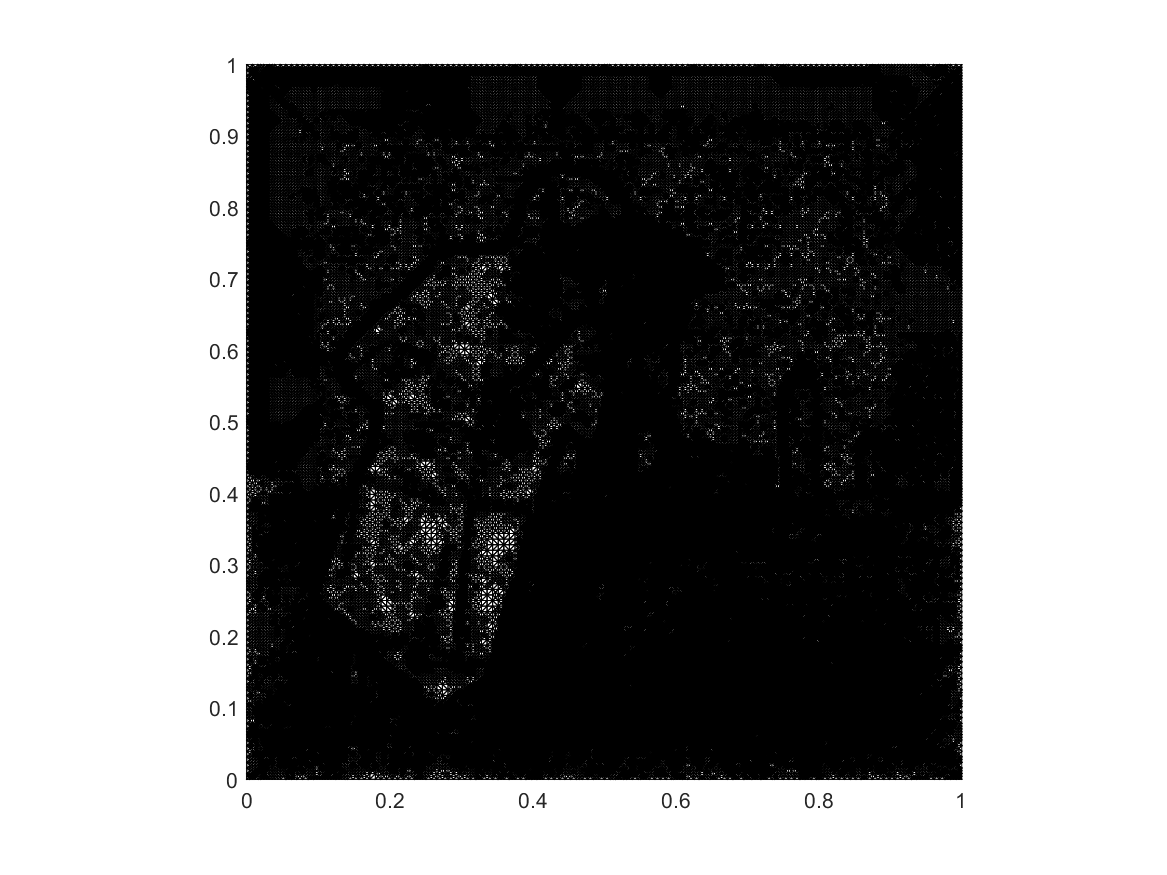
\includegraphics[trim = 100 30 80 20, clip, width=\linewidth]
      {pictures/chapExperiments/secGrayscale/cam/adaptive/lvl21/triangulation.png}
    \label{fig:camLvl21Triang}
  \end{subfigure}
  \quad
  \begin{subfigure}[b]{.48\linewidth}
    \centering
    \caption{Lösung Level 21}
    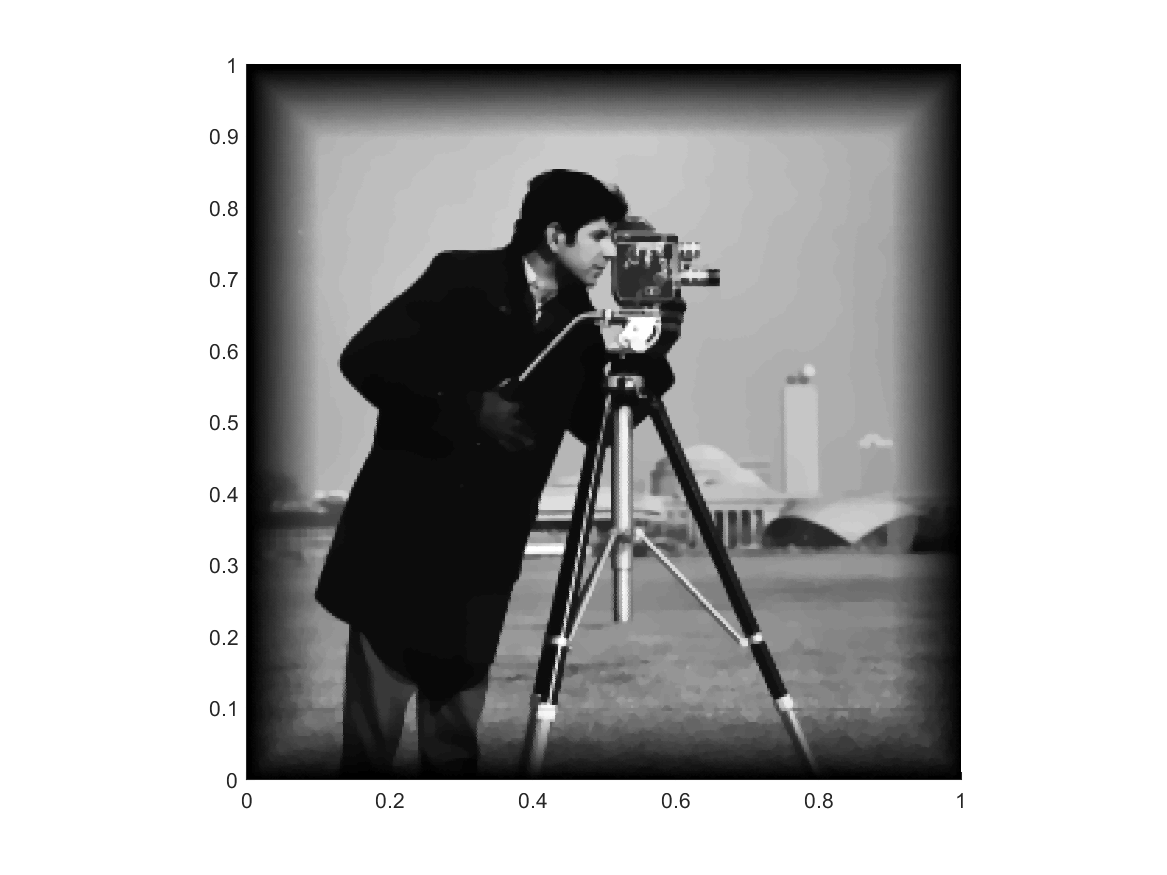
\includegraphics[trim = 100 30 80 20, clip, width=\linewidth]
      {pictures/chapExperiments/secGrayscale/cam/adaptive/lvl21/solutionGrayscale.png}
    \label{fig:camLvl21Sol}
  \end{subfigure}
  \caption{Triangulierung und Lösung für Eingangssignal \texttt{cameraman}.}
  \label{fig:camTriang}
\end{figure}

vielleicht auch als 4x4 mit darunter noch das gleiche für das letzte lvl 21
hier noch die Freiheitsgrade ergänzen

darüber reden, dass der schwarze rand den gewünschte effekt und damit weniger
richtung rand verfeinert wird (was unnötig wäre, künstlich, weil 0 Randdaten)

selbst auf lvl 21 kann man. trotz closure, erahnen, wo die farbe sehr monoton 
war und weniger verfeinert wurde, was gut ist, da man das genau so möchte

==================

abschweif zu denoise example aus intro hier erklären

==================

Für die Funktion
\begin{align*}
  u_\textrm{C}(r)\coloneqq 
  \begin{cases}
    1, & \text{wenn } 0\leq r\leq\frac{1-\beta}{2},\\
    -\frac{1}{\beta}r + \frac{1+\beta}{2\beta}, & 
    \text{wenn } \frac{1-\beta}{2}\leq r\leq \frac{1+\beta}{2},\\
    0, & \text{wenn } \frac{1+\beta}{2}\leq r,
  \end{cases}
\end{align*}
erhält man mit der Wahl
\begin{align*}
  \sgn&(\partial_r u_\textrm{C}(r)) \\
  &\coloneqq 
  \begin{cases}
    \frac{4}{1-\beta}r\left(\frac{1}{1-\beta}r -1\right)\!, &
    \text{wenn } 0\leq r\leq\frac{1-\beta}{2},\\
    -1, & \text{wenn } \frac{1-\beta}{2}\leq r\leq \frac{1+\beta}{2},\\
    \frac{4}{(\beta-1)^3}
    \left( 4r^3-3(\beta+3)r^2 +6(\beta+1)r-3\beta-1\right)\!, & 
    \text{wenn } \frac{1+\beta}{2}\leq r\leq 1,
  \end{cases}
\end{align*}
die rechte Seite
\begin{align*}
  f_\textrm{C}(r)\coloneqq 
  \begin{cases}
    \alpha - \frac{4}{1-\beta}\left(\frac{3}{1-\beta}r - 2\right)\!, &
    \text{wenn } 0\leq r\leq\frac{1-\beta}{2},\\
    -\frac{\alpha}{\beta}\left( r-\frac{1+\beta}{2} \right) +\frac{1}{r}, & 
    \text{wenn } \frac{1-\beta}{2}\leq r\leq \frac{1+\beta}{2},\\
    \frac{-4}{(\beta-1)^3}
    \left( 16r^2 -9(\beta+3)r + 12(\beta+1) - \frac{3\beta+1}{r}\right)\!, & 
    \text{wenn } \frac{1+\beta}{2}\leq r\leq 1.
  \end{cases}
\end{align*}

\begin{align*}
  \partial_r f_\textrm{C}(r) &= 
  \begin{cases}
    -\frac{12}{(1-\beta)^2},&\text{wenn }0\leq r\leq\frac{1-\beta}{2},\\
    -\frac{\alpha}{\beta}-\frac{1}{r^2},&
    \text{wenn } \frac{1-\beta}{2}\leq r\leq \frac{1+\beta}{2},\\
    -\frac{4}{(1-\beta)^3}\left( 32r-9(\beta+3)+\frac{3\beta+1}{r^2} \right)\!,&
    \text{wenn } \frac{1+\beta}{2}\leq r\leq 1,\\
  \end{cases}
\end{align*}
\begin{align*}
  \partial_r u_\textrm{C}(r) &= 
  \begin{cases}
    0,&\text{wenn }0\leq r\leq\frac{1-\beta}{2},\\
    -\frac{1}{\beta},&
    \text{wenn } \frac{1-\beta}{2}\leq r\leq \frac{1+\beta}{2},\\
    0,&\text{wenn } \frac{1+\beta}{2}\leq r,
  \end{cases}
\end{align*}

$u_\textrm{C}$ ist eine stetige Approximation von
\begin{align*}
  u_\textrm{DC}(r)\coloneqq 
  \begin{cases}
    1, & \text{wenn } 0\leq r\leq\frac{1}{2},\\
    0, & \text{wenn } \frac{1}{2}\leq r,
  \end{cases}
\end{align*}

\begin{figure}[p]
  \centering
  \begin{subfigure}[b]{.48\linewidth}
    \centering
    \caption{Insi circle stetig entlang der Achsen}
    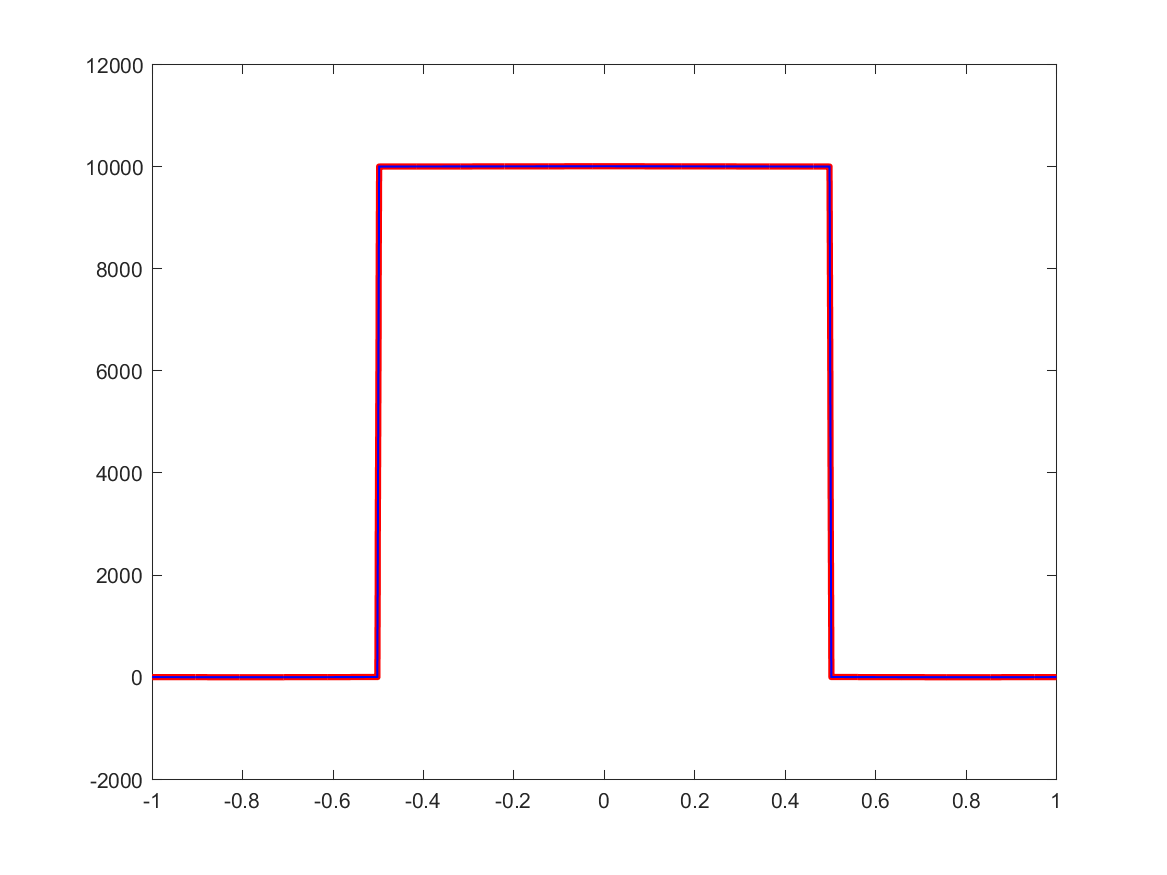
\includegraphics[trim = 40 30 50 20, clip, width=\linewidth]
      {pictures/chapExperiments/secGrayscale/circ/cont/inSiAxis.png}
    \label{fig:circContInSiAxis}
  \end{subfigure}
  \quad
  \begin{subfigure}[b]{.48\linewidth}
    \centering
    \caption{Exakte Lsg circle stetig entlang der Achsen}
    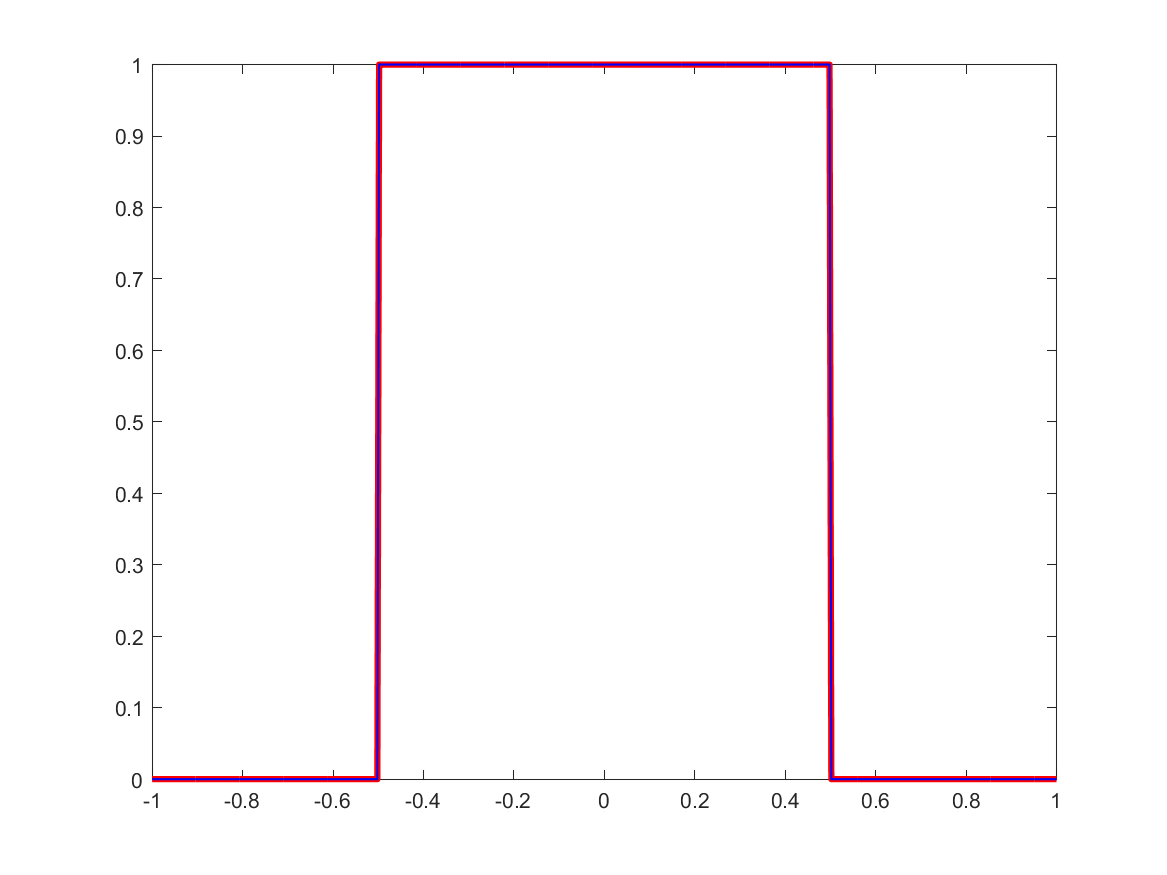
\includegraphics[trim = 40 30 50 20, clip, width=\linewidth]
      {pictures/chapExperiments/secGrayscale/circ/cont/exactSolutionAxis.png}
    \label{fig:circContExactSolAxis}
  \end{subfigure}
  \caption{InSi und exakte Lösung circle stetig entlang der Achsen.}
  \label{fig:circContPlotsAxis}
\end{figure}

\begin{figure}[p]
  \centering
  \begin{subfigure}[b]{.48\linewidth}
    \centering
    \caption{adaptive Konvergenz vergleich stetig und unstetig}
    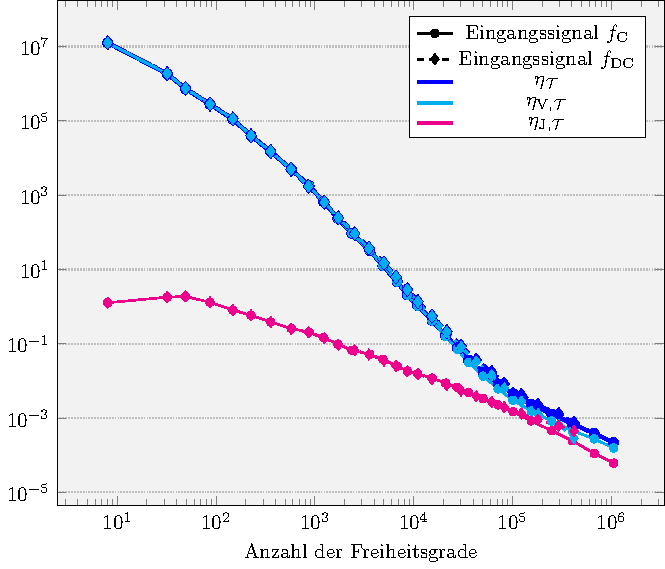
\includegraphics[width=\linewidth]
      {pictures/chapExperiments/secGrayscale/circ/convAdap.pdf}
    \label{fig:circConvAdaptive}
  \end{subfigure}
  \quad
  \begin{subfigure}[b]{.48\linewidth}
    \centering
    \caption{uniforme Konvergenz vergleich stetig und unstetig}
    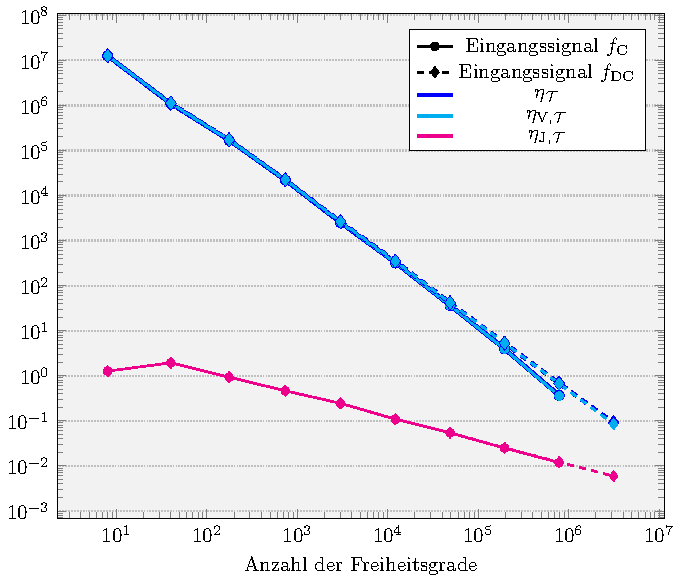
\includegraphics[width=\linewidth]
      {pictures/chapExperiments/secGrayscale/circ/convUnif.pdf}
    \label{fig:circConvUniform}
  \end{subfigure}
  \caption{adptive und uniformer Vergleich für circle stetig und unstetig}
  \label{fig:circConvComparison}
\end{figure}

\begin{figure}[p]
  \centering
  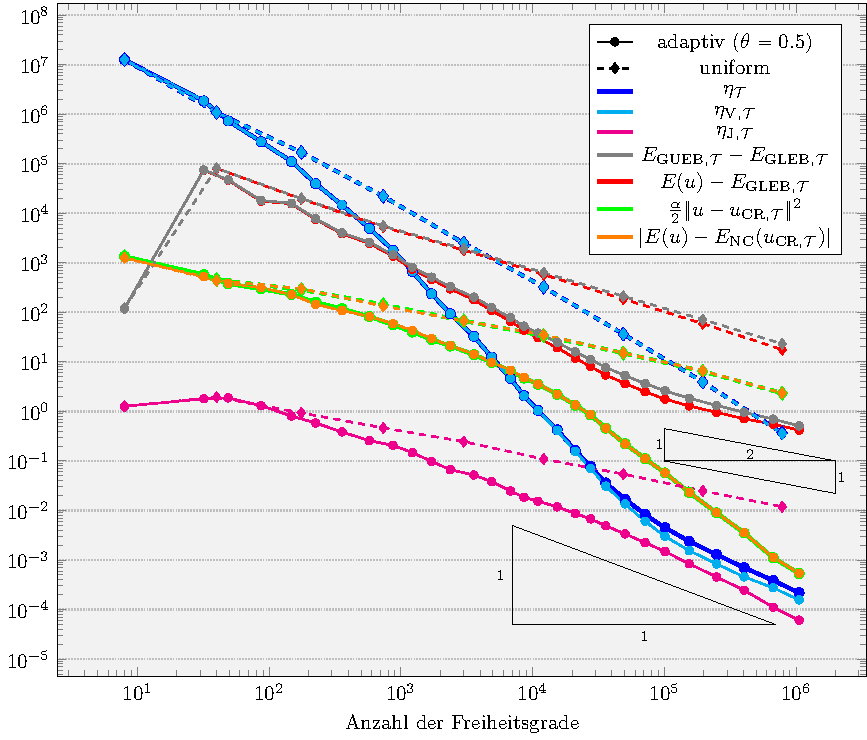
\includegraphics[width=\linewidth]
    {pictures/chapExperiments/secGrayscale/circ/convCont.pdf}
  \caption{Ergebnisse für Eingangssignal circle stetig.}
  \label{fig:circContConvergence}
\end{figure}

\begin{figure}[p]
  \centering
  \begin{subfigure}[b]{.48\linewidth}
    \centering
    \caption{Triangulierung stetig Level 17}
    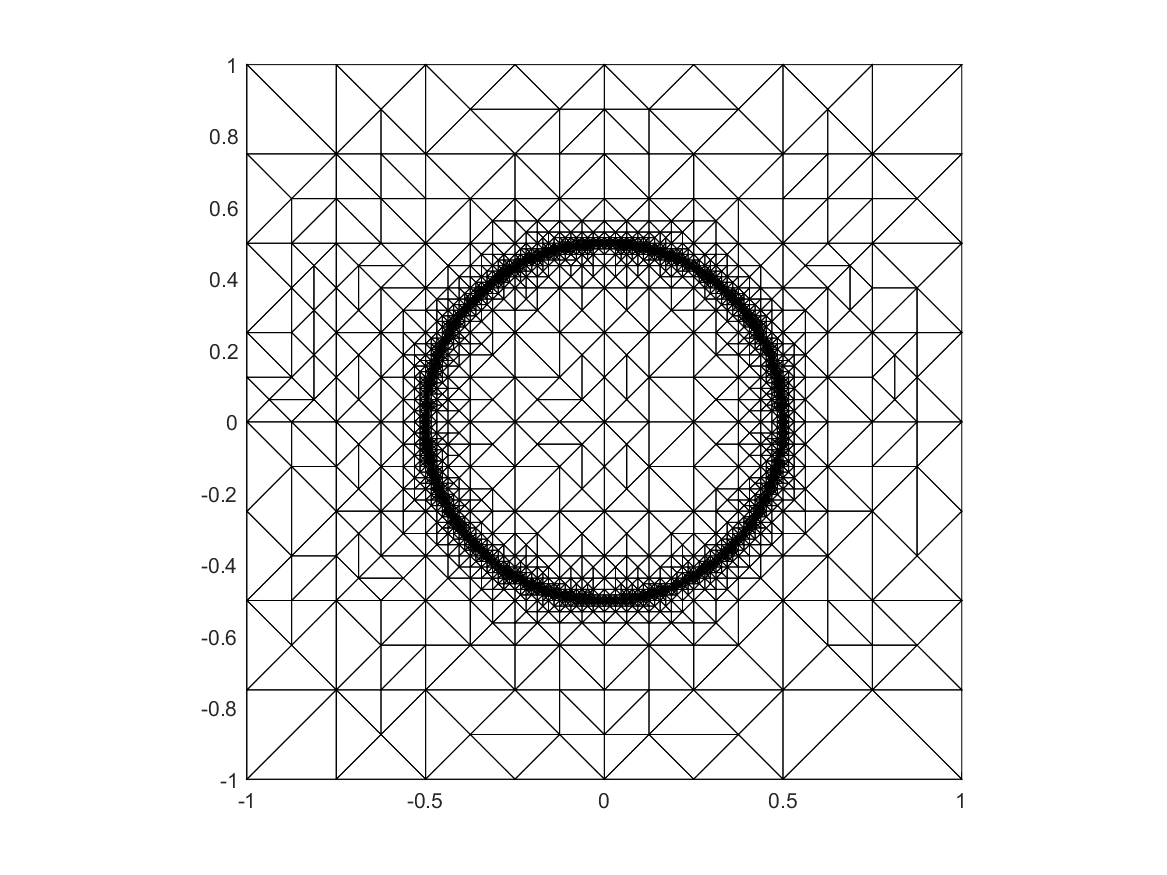
\includegraphics[trim = 100 30 80 20, clip, width=\linewidth]
      {pictures/chapExperiments/secGrayscale/circ/cont/adaptive/lvl17/triangulation.png}
    \label{fig:circContLvl17Triang}
  \end{subfigure}
  \quad
  \begin{subfigure}[b]{.48\linewidth}
    \centering
    \caption{Triangulierung unstetig Level 17}
    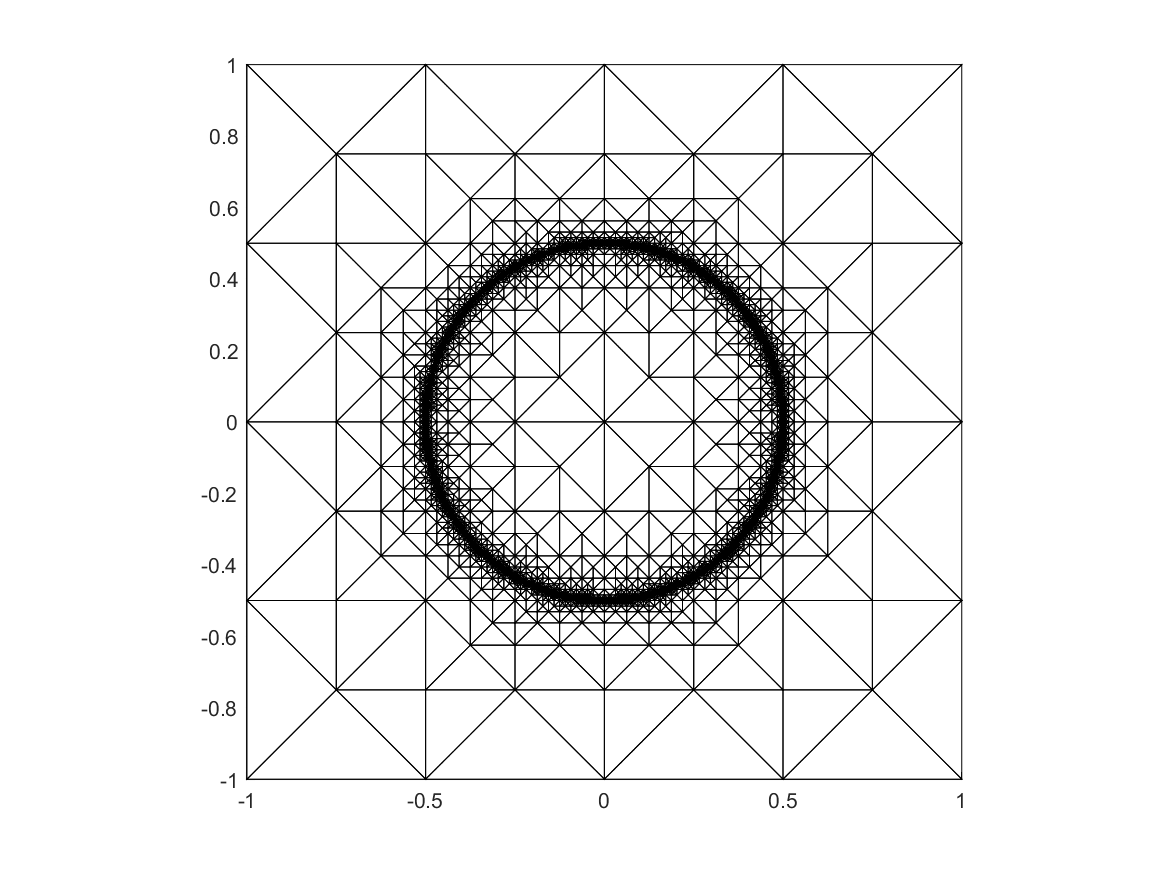
\includegraphics[trim = 100 30 80 20, clip, width=\linewidth]
      {pictures/chapExperiments/secGrayscale/circ/disc/adaptive/lvl17/triangulation.png}
    \label{fig:circDiscLvl17Triang}
  \end{subfigure}

  \begin{subfigure}[b]{.48\linewidth}
    \centering
    \caption{Triangulierung stetig Level Final}
    \includegraphics[trim = 100 30 80 20, clip, width=\linewidth]
      {pictures/chapExperiments/secGrayscale/circ/cont/adaptive/lvl25/triangulation.png}
    \label{fig:circContFinalTriang}
  \end{subfigure}
  \quad
  \begin{subfigure}[b]{.48\linewidth}
    \centering
    \caption{Triangulierung unstetig Level Final}
    \includegraphics[trim = 100 30 80 20, clip, width=\linewidth]
      {pictures/chapExperiments/secGrayscale/circ/disc/adaptive/lvl23/triangulation.png}
    \label{fig:circDiscFinalTriang}
  \end{subfigure}
  \caption{Triangulierung für InSi circle stetig und unstetig.}
  \label{fig:circleTriang}
\end{figure}

\begin{figure}[p]
  \centering
  \begin{subfigure}[b]{.48\linewidth}
    \centering
    \caption{Lösung circ stetig}
    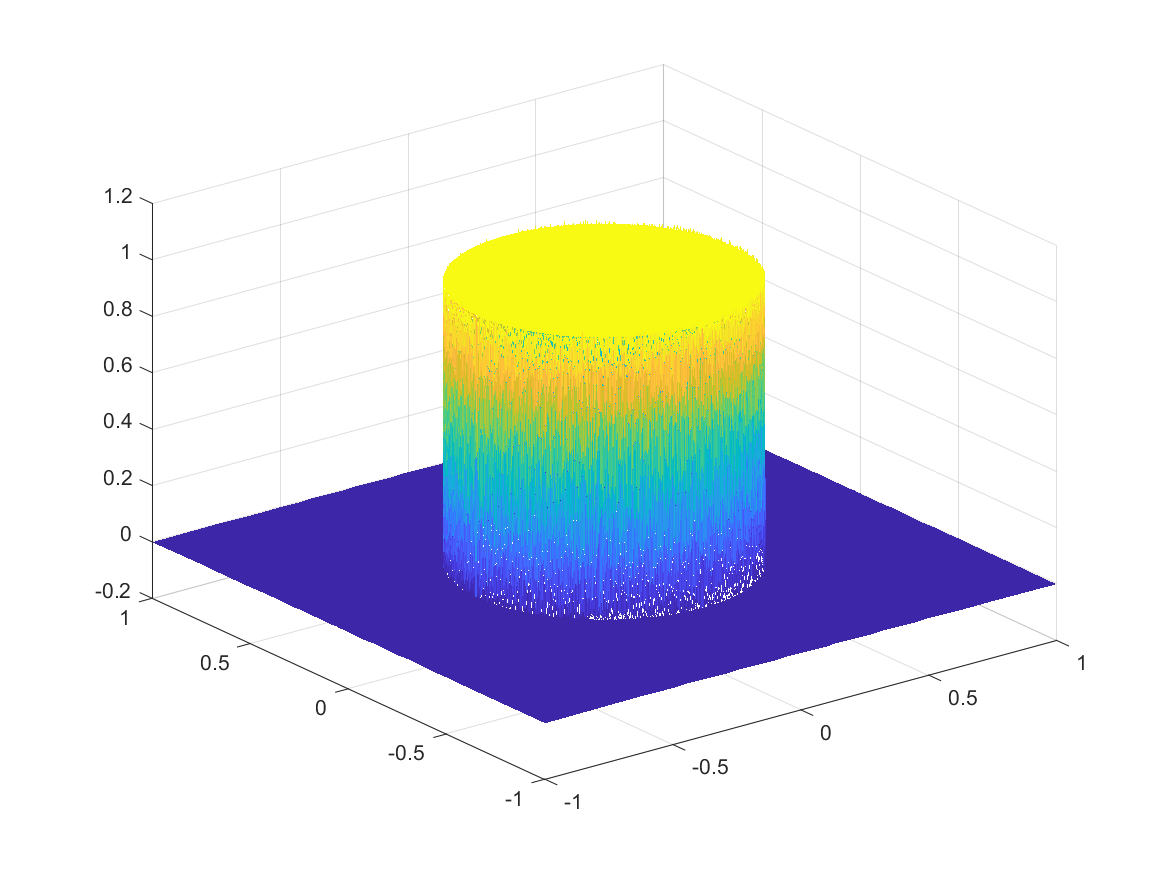
\includegraphics[trim = 40 30 30 30, clip, width=\linewidth]
      {pictures/chapExperiments/secGrayscale/circ/cont/adaptive/lvl25/solution.png}
    \label{fig:circContSol}
  \end{subfigure}
  \quad
  \begin{subfigure}[b]{.48\linewidth}
    \centering
    \caption{Lösuns stetig final entlang der Achsen}
    \includegraphics[trim = 50 30 50 20, clip, width=\linewidth]
      {pictures/chapExperiments/secGrayscale/circ/cont/adaptive/lvl25/solutionAxis.png}
    \label{fig:circContSolAxis}
  \end{subfigure}

  \begin{subfigure}[b]{.48\linewidth}
    \centering
    \caption{Lösung circ unstetig}
    \includegraphics[trim = 40 30 30 30, clip, width=\linewidth]
      {pictures/chapExperiments/secGrayscale/circ/disc/adaptive/lvl23/solution.png}
    \label{fig:circDiscSol}
  \end{subfigure}
  \quad
  \begin{subfigure}[b]{.48\linewidth}
    \centering
    \caption{Lösuns unstetig final entlang der Achsen}
    \includegraphics[trim = 50 30 50 20, clip, width=\linewidth]
      {pictures/chapExperiments/secGrayscale/circ/disc/adaptive/lvl23/solutionAxis.png}
    \label{fig:circDiscSolAxis}
  \end{subfigure}
  \caption{Lösung für Eingangssignal circle steig und unstetig.}
  \label{fig:circleSol}
\end{figure}

\todo[inline]{circ cont insi für alpha 1e4 und beta 1/100 entlang der Achsen}
\Cref{fig:circDiscSolAxis} natürlich Sprung bei 1/2, nur geplottet aus
Implementierungsgründen. Es geht darum zu sehen, dass die ansonsten, insb
die Höhen, gleich sind

\Cref{fig:circConvComparison} vlt besser ohne Dreiecke, weil die sieht man
ja alle dann in \Cref{fig:circContConvergence}.

In \Cref{fig:circContPlotsAxis} sehen wir, wie nah diese stetige Funktion 
an der unstetigen Indikatorfunktion für den Kreis liegt.
Außerdem sehen wir dort auch wieder das erwarte Verhalten, dass das InSi
alpha mal die exakte Lösung zu sein scheint, da alpha hier groß

zum abschluss zu approximation von white circle mit stetigeer funktion (plots
dementsprechend

betonen, dass das natürlich kein Graufarbenbild ist, aber natürlich einfach
ind das entsprechende Setting übertragen werden kann.
Das abschließende Beispiel ist zwar dem Programm nicht als Graufarbenbild 
gegeben, aber es ist ein simples Beispiel das entlang einer Teilmenge des
$\Rbb^2$ unstetig. Plot. Und hier statt Plot entlang der Achen jeweils
den Plot als Graufarbenbild. (sowohl für cont als discont Funktion)

  - circle stuff, etas sind vergleichbar (was gut, weil so erwarte)

diskontinuierliche function und eine stetige approximation dieser

welche Plots: 
alle sachen, die für cont und discont beide geplottet werden können, in einen
plot. vielleicht nebeneinander mit subfigures, links adaptiv, rechts uniform.
Falls die Sachen so gleich sind, wie sie hoffentlich sein sollten, wieder
die hintere linie dick und die vordere weniger dick, wie den einen tau
convergence plot. 
als letztes, nachdem klargestellt wurde, dass alle Raten die für cont und
discont plotbar sind im wesentlichen gleich sind, adaptiv/uniform standart plot
für continuous plot, mit vermerk, dass dies möglicherweise etwas über die nicht
plotbaren sachen für discont problem aussagt

vielleicht auch nochmal triangulierungen, ähnliche freiheitsgrade für cont 
und discont, die hoffenlich sehr ähnlich sein sollten (mglw geht sogar das 
höchste level hierfür), Triangulierung auf ähnliche Freiheitsgrade achten

Triangulierung ja, Lösung nur, wenn die nicht einfach genau so aussehen, wie
man es erwartet

betonen, dass man als stückweisen Gradienten für die rechte seite der nicht 
stetigen Variante schlicht 0 genommen hat, unabhänig davon, dass das
kein schwacher gradient ist


\section{Fazit und Ausblick}

aus altem Auswertungen.tex (neues: s. Storn, Puttkams)

In diesen Abschnitt werten wir die in \Cref{chap:experiments} erhaltenen
Ergebnisse aus.

\todo[inline]{folgendes weniger ausführlich einbringen, wohl
auch eher im Auswertungskapitel ,,in Bartels wird in
citeEntsprechendesLemma die garantierte Rate für \ldots bewiesen. In unseren
Experimenten \ldots}

====================

\Cref{fig:parTauNoConvergence} legt nahe, über nicht konstante Wahlen für
$\tau$ nachzu\-denken, die mög\-lich\-er\-wei\-se das alternierende Verhalten in
\Cref{fig:parTauNoConvergenceEnergy} verhindern könnte

====================

Punkte auf die bei den Auswertungen eingegangen werden sollte

Raten

Verfeinerungsindikator
AUSBLICK (vielleicht in die Arbeit schreiben)
  
  Randdaten verallgemeinern
    nochmal aufschreiben wo CR10 angenommen wird und eventuell darauf verweisen 
    im Ausblick (bis dahin notieren welche Funktionen und in welchem Maß)
    (in solvePrimalDualFormulation zum Erstellen der rechten Seite)
    
  Bartels Code anpassen und vergleicen

BEI allen Triangulierungsbildern die Freiheitsgrade ergänzen, mglsweise auch
bei allen Lösungsplots
